\documentclass[10pt,twocolumn,a4paper]{article}

\usepackage[english]{babel}
\usepackage[utf8]{inputenc}
\usepackage[T1]{fontenc}

\IfFileExists{sourcesanspro.sty}{%
  \usepackage[default,semibold]{sourcesanspro}%
}{%
  \usepackage{helvet}%
}
\renewcommand{\familydefault}{\sfdefault}
\usepackage{newtxsf}

\usepackage{amsmath,amssymb}
\usepackage{graphicx}
\usepackage{booktabs}
\usepackage{array,tabularx}
\usepackage[a4paper,margin=0.75in,top=0.9in,bottom=0.9in,
            columnsep=0.3in,headheight=32pt,headsep=12pt]{geometry}
\usepackage{setspace}
\setstretch{1.05}
\usepackage{xcolor}
\definecolor{headdark}{RGB}{27,52,73}
\definecolor{headmid}{RGB}{60,80,100}
\definecolor{headrule}{RGB}{200,205,215}
\usepackage{titlesec}
% Section numbers stay so the text can cite them.
\titleformat{\section}{\normalsize\bfseries\color{headmid}}{\thesection.}{0.55em}{\MakeUppercase}
\titleformat{\subsection}{\normalsize\bfseries}{\thesubsection}{0.5em}{}
\titleformat{\subsubsection}{\normalsize\bfseries\itshape}{}{0pt}{}
\titlespacing*{\section}{0pt}{1.1\baselineskip}{0.35\baselineskip}
\titlespacing*{\subsection}{0pt}{0.75\baselineskip}{0.20\baselineskip}
\titlespacing*{\subsubsection}{0pt}{0.55\baselineskip}{0.15\baselineskip}
\setcounter{secnumdepth}{2}

\usepackage[hidelinks]{hyperref}
\usepackage{microtype}
\emergencystretch=3em
\hyphenpenalty=1000
\tolerance=1500
\hyphenation{Table table Tables tables}
\usepackage{caption}
\captionsetup{font=small,labelfont={bf,color=headmid},belowskip=4pt,
              aboveskip=6pt,justification=justified,singlelinecheck=false,
              skip=4pt}
\usepackage{stfloats}
\usepackage{placeins}
\usepackage{float}
\renewcommand{\topfraction}{0.9}
\renewcommand{\dbltopfraction}{0.9}
\renewcommand{\textfraction}{0.05}
\renewcommand{\floatpagefraction}{0.8}
\renewcommand{\dblfloatpagefraction}{0.8}
\setcounter{topnumber}{3}
\setcounter{dbltopnumber}{3}

\usepackage[numbers,sort&compress,super,square]{natbib}
\bibliographystyle{vancouver}

\newcommand{\DIF}{\mathrm{DIF}}
\newcommand{\neff}{n_{\mathrm{eff}}}
\newcommand{\tabwidth}{\columnwidth}
\newcommand{\cellbr}[2]{\begin{tabular}[t]{@{}c@{}}#1\\#2\end{tabular}}
% Every table body is \small, with the same column padding. A one-column
% table fills \columnwidth. A full-width table fills \textwidth, which in
% this layout is the left edge of the first column to the right edge of
% the second. Captions are set before \tabbody so they are not shrunk twice.
\newcommand{\tabbody}{\small\setlength{\tabcolsep}{3.5pt}\renewcommand{\arraystretch}{1.08}}
\newcommand{\onetab}{\renewcommand{\tabwidth}{\columnwidth}\tabbody}
\newcommand{\fulltab}{\renewcommand{\tabwidth}{\textwidth}\tabbody}
\newbox\highlightbox
\newenvironment{highlights}{\setbox\highlightbox=\vbox\bgroup\begin{itemize}}{\end{itemize}\egroup}
\renewenvironment{abstract}{\par\vspace{3pt}\noindent\ignorespaces}{\par}
\newcommand{\Npool}{55}
\newcommand{\NinframeRes}{5}
\newcommand{\Ninframe}{16}
\newcommand{\ResRate}{31}
\newcommand{\DiffBenign}{1.4}
\newcommand{\AucIid}{0.93}
\newcommand{\LrdH}{0.8}
\newcommand{\NsfTwo}{31}
\newcommand{\NsfTwoRes}{20}
\newcommand{\NsfTwoStrict}{18}
\newcommand{\NsfTwoUnres}{11}
\newcommand{\NsfTwoNone}{15}
\newcommand{\NsfTwoSeedFold}{3}
\newcommand{\NsfTwoTestCI}{2}

% Generated by scripts/make_tables.py from results/ and diagnostics/. Do not edit.
\newcommand{\FprBothNaive}{0.59\pm0.02}
\newcommand{\FprBothEss}{0.92\pm0.01}
\newcommand{\FprBothMbb}{0.87\pm0.01}
\newcommand{\FprLrdEss}{0.55\pm0.02}
\newcommand{\FprLrdMbb}{0.60\pm0.02}
\newcommand{\AucCtrlNaive}{0.93\pm0.01}
\newcommand{\AucCtrlMbb}{0.92\pm0.01}
\newcommand{\RecallCampNaive}{0.70\pm0.02}
\newcommand{\RecallCampEss}{0.70\pm0.02}
\newcommand{\RecallCampEssCond}{0.95\pm0.01}
\newcommand{\RecallCampComp}{0.74}
\newcommand{\RecallCampEssPt}{0.70}
\newcommand{\RecallCampEssCondPt}{0.95}
\newcommand{\RecallBothNaive}{0.32\pm0.02}
\newcommand{\RecallBothEss}{0.54\pm0.02}
\newcommand{\RecallBothNaiveCond}{0.45\pm0.03}
\newcommand{\RecallBothEssCond}{0.76\pm0.02}
\newcommand{\RecallBothComp}{0.72}
\newcommand{\RecallEp}{0.22\pm0.02}
\newcommand{\RecallEpCond}{0.30\pm0.02}
\newcommand{\AucBothNaive}{0.26\pm0.02}
\newcommand{\AucBothMbb}{0.56\pm0.02}
\newcommand{\AucBothNaiveCond}{0.36\pm0.03}
\newcommand{\AucBothMbbCond}{0.78\pm0.02}
\newcommand{\AucCampNaiveCond}{0.93\pm0.01}
\newcommand{\AucCampMbbCond}{0.83\pm0.02}
\newcommand{\RecallNtwNaive}{0.48\pm0.02}
\newcommand{\RecallNtwEss}{0.88\pm0.01}
\newcommand{\AucNtwNaive}{0.37\pm0.02}
\newcommand{\AucNtwMbb}{0.86\pm0.01}
\newcommand{\FprNtwEss}{0.95\pm0.01}
\newcommand{\FprNtwNaive}{0.58\pm0.02}
\newcommand{\AucCampNtwNaive}{0.91\pm0.01}
\newcommand{\AucCampNtwMbb}{0.89\pm0.01}
\newcommand{\AucCtrlBhiNaive}{0.936}
\newcommand{\AucCtrlBhiMbb}{0.926}
\newcommand{\AucCtrlBloNaive}{0.934}
\newcommand{\AucCtrlBloMbb}{0.924}
\newcommand{\AucLrdBjk}{0.54}
\newcommand{\AucLrdBjkBhi}{0.49}
\newcommand{\SplitTempNaive}{0.60\pm0.02}
\newcommand{\SplitTempEss}{0.95\pm0.01}
\newcommand{\SplitShuf}{0.71\pm0.02}
\newcommand{\SplitShufEss}{0.71\pm0.02}
\newcommand{\SplitRestNaive}{0.71\pm0.02}
\newcommand{\SplitRestEss}{0.94\pm0.01}
\newcommand{\TauTemp}{19.5}
\newcommand{\TauShuf}{1.0}
\newcommand{\TauRest}{10.2}
\newcommand{\SfOnePop}{0.83}
\newcommand{\SfOneCond}{0.93}
\newcommand{\SfOneWilson}{0.95}
\newcommand{\EpEssFive}{0.87}
\newcommand{\EpEssTwenty}{0.94}
\newcommand{\PktQGeyer}{2.1}
\newcommand{\PktQBatch}{1.8}
\newcommand{\PktQNeff}{43{,}576}
\newcommand{\PktMidGeyer}{163.4}
\newcommand{\PktMidBatch}{26.9}
\newcommand{\PktLateGeyer}{152.0}
\newcommand{\PktLateBatch}{16.5}
\newcommand{\PktRangeLo}{16.5}
\newcommand{\PktRangeHi}{163.4}
\newcommand{\PktFactorMid}{6.1}
\newcommand{\PktFactorLate}{9.2}
\newcommand{\FlowBpsMon}{1}
\newcommand{\FlowBpsTue}{1}
\newcommand{\FlowBpsWed}{64}
\newcommand{\WinQMed}{3.5}
\newcommand{\WinQn}{3}
\newcommand{\WinAllMed}{96}
\newcommand{\FlowQualMed}{3.4}
\newcommand{\FlowShuffleMed}{17.5}
\newcommand{\BlkBothOne}{0.78\pm0.02}
\newcommand{\BlkBothTwo}{0.76\pm0.02}
\newcommand{\BlkBothFour}{0.75\pm0.02}
\newcommand{\BlkCampOne}{0.85\pm0.02}
\newcommand{\BlkCampTwo}{0.83\pm0.02}
\newcommand{\BlkCampFour}{0.81\pm0.02}
\newcommand{\BlkLOne}{132}
\newcommand{\BlkLFour}{214}
\newcommand{\WidFprBoth}{0.97}
\newcommand{\WidFprBothSmall}{0.96}
\newcommand{\WidRecBoth}{0.71}
\newcommand{\WidRecBothSmall}{0.48}
\newcommand{\WidRecCamp}{0.99}
\newcommand{\WidNeffRecBoth}{1.99}
\newcommand{\WidNeffRecBothSmall}{4.29}
\newcommand{\WidNeffFprBoth}{1.06}
\newcommand{\WidFprBothNaive}{0.40}
\newcommand{\WidCampCount}{5.1}
\newcommand{\AucBootRatioBoth}{0.89}
\newcommand{\AucBootRatioBothSmall}{0.60}
\newcommand{\AucBootRatioCtrl}{1.02}
\newcommand{\AucBootRatioCtrlSmall}{0.96}
\newcommand{\AucOffsetBoth}{-0.12}
\newcommand{\AucCovRefBoth}{0.87}
\newcommand{\AucCovRecBoth}{0.86}
\newcommand{\AucRecentreGap}{-0.003}
\newcommand{\AucLBoth}{524}
\newcommand{\AucNbBoth}{38}
\newcommand{\TraceDurEssFive}{0.86\pm0.02}
\newcommand{\TraceDurEssTwenty}{0.92\pm0.01}
\newcommand{\TraceDurNaiveFive}{0.73\pm0.02}
\newcommand{\RecallClockSubFive}{0.50\pm0.02}
\newcommand{\RecallClockMisFive}{0.50\pm0.02}
\newcommand{\RecallClockSubTwenty}{0.87\pm0.01}
\newcommand{\RecallClockMisTwenty}{0.86\pm0.02}
\newcommand{\MonIfFprRatio}{1.55}
\newcommand{\MonIfFprDif}{2.37}
\newcommand{\WedIfFprDif}{45.64}
\newcommand{\WedAucFlip}{-0.0073}
\newcommand{\HGridLo}{0.55}
\newcommand{\HGridHi}{0.9}
\newcommand{\HGridN}{5}
\newcommand{\FprHLo}{0.96\pm0.01}
\newcommand{\FprHSix}{0.93\pm0.01}
\newcommand{\FprHSeven}{0.82\pm0.02}
\newcommand{\FprHNine}{0.33\pm0.02}
\newcommand{\FprHSevenMbb}{0.78}
\newcommand{\FprHEightMbb}{0.60}
\newcommand{\NeffHLo}{1087}
\newcommand{\NeffHNine}{64}
\newcommand{\GateAlarmNine}{0.92}
\newcommand{\GateScoreNine}{0.11}
\newcommand{\GateAlarmEight}{0.99}
\newcommand{\GateScoreEight}{0.40}
\newcommand{\GateScoreSeven}{0.89}
\newcommand{\GateScoreSix}{1.00}
\newcommand{\TauAlarmNine}{3.6}
\newcommand{\TauScoreNine}{74}
\newcommand{\GateR}{500}
\newcommand{\GateScoreNeffOnlyNine}{0.63}


\pagestyle{plain}
\hypersetup{
  pdftitle={When Confidence Intervals Assume Independence: Dependence-Aware Intervals for Intrusion-Detection Evaluation},
  pdfauthor={Soheib Cherih, Sabri Lyazid, and Okba Kazar}
}

\begin{document}

\twocolumn[{%
  {\raggedright
    \noindent{\LARGE\bfseries\color{headdark}%
      When Confidence Intervals Assume Independence:\par
      Dependence-Aware Intervals for Intrusion-Detection Evaluation\par}
    \vspace{10pt}
    \noindent{\normalsize\bfseries%
      Soheib Cherih,\textsuperscript{1,*}\;
      Sabri Lyazid\textsuperscript{1}\;
      Okba Kazar\textsuperscript{2}\par}
    \vspace{3pt}
    \noindent{\footnotesize\itshape%
      \textsuperscript{1}Intelligent Systems and Cognitive Computing
      Laboratory (ISCC), Department of Computer Science,
      University of Mohamed El Bachir El Ibrahimi,
      Bordj Bou Arreridj, Algeria.\par}
    \vspace{1pt}
    \noindent{\footnotesize\itshape%
      \textsuperscript{2}College of Arts, Sciences \& Information Technology,
      Department of Computer Science, University of Kalba,
      Sharjah, United Arab Emirates.\par}
    \vspace{2pt}
    \noindent{\footnotesize%
      \textsuperscript{*}Corresponding author. Soheib Cherih;
      e-mail:
      \href{mailto:souhaib.cherrih@univ-bba.dz}{souhaib.cherrih@univ-bba.dz}.
      Co-authors: Sabri Lyazid,
      \href{mailto:lyazid.sabri@univ-bba.dz}{lyazid.sabri@univ-bba.dz};
      Okba Kazar,
      \href{mailto:Okba.Kazar@ukb.ac.ae}{Okba.Kazar@ukb.ac.ae}.\par}
  }
  \vspace{10pt}
  {\color{headrule}\hrule height 0.6pt}
  \vspace{8pt}
  {\raggedright
    \noindent{\large\bfseries\color{headdark}Abstract}\par
    \vspace{3pt}
\begin{abstract}
On the clean Monday CICIDS2017 prefix, isolation-forest alarm dependence widens the false-positive interval $\MonIfFprRatio\times$ (dependence-inflation factor $\MonIfFprDif$), changing one close Wednesday ranking but not the large gaps.
The intervals differ by metric: an ESS-adjusted Wilson plug-in for the false-positive rate, an ESS plug-in on the attack subsequence for recall, a moving-block bootstrap of Mann--Whitney for AUC.
At $n{=}20000$ in the strongest short-memory cell they cover at $\FprNtwEss$, $\RecallNtwEss$ and $\AucNtwMbb$; on a resampled Monday Flow Duration trace, $\TraceDurEssFive$ and $\TraceDurEssTwenty$ at $n{=}5000$ and $20000$.
Across $\HGridN$ Hurst exponents it holds to $H{=}0.6$ ($\FprHSix$), then degrades monotonically to $\FprLrdEss$ at $H{=}\LrdH$ and $\FprHNine$ at $H{=}\HGridHi$.
The estimator-agreement gate must be read on the benign score series, not the alarm indicator the interval uses: on the indicator it admits $\GateAlarmNine$ of replicates at $H{=}\HGridHi$, where coverage is $\FprHNine$, and on the score series $\GateScoreNine$.
Report ESS--Wilson when those estimators agree and $\neff$ is at least 50; otherwise report $\neff$ and no interval.
Of \Npool{} screened records \NsfTwoRes{} could be coded, \NsfTwoNone{} reporting no uncertainty; the time-aware frame resolved \NinframeRes{} of \Ninframe{} (\ResRate\%), an illustration, not a prevalence claim.
\end{abstract}
  \smallskip
  \noindent\textbf{Keywords.}\enspace effective sample size; intrusion detection; confidence
  intervals; serial dependence; block bootstrap; evaluation methodology; autocorrelation.
  \vspace{6pt}
  {\color{headrule}\hrule height 0.6pt}
  \vspace{10pt}
  }
}]

\thispagestyle{plain}
\begin{highlights}
\item Monday alarm dependence widens one false-positive interval by \MonIfFprRatio
\item False-positive, recall, and AUC intervals are different constructions
\item ESS--Wilson holds to $H{=}0.6$ and degrades monotonically above it
\item One close Wednesday ranking flips; large detector gaps do not
\item Read the agreement gate on scores: the alarm indicator hides long memory
\end{highlights}

\section{Background and Significance}
Learning-based intrusion-detection papers report a confidence interval on a flow- or window-level
test metric and read non-overlapping intervals as evidence that one detector beats
another~\citep{arp2022dos,lew2026deployment}. Overlap is not that test, even for independent
estimates~\citep{schenker2001overlap}. A
nominal-$n$ interval on that metric --- an i.i.d.\ bootstrap of the test rows, or a Wald or Wilson
interval~\citep{wilson1927probable,brown2001interval,mcgrath2024binomial} that takes the flow or window count as $n$ ---
treats those rows as exchangeable. A fold-level $t$-test or a Wilcoxon test over
runs~\citep{wilcoxon1945individual} is a different estimand: the sample is the runs,
not the telemetry. This paper is about the first. Benign traffic is autocorrelated and
self-similar on the timescales Paxson and Floyd documented~\citep{paxson1995failure,leland1994self}.
Later backbone traces show that long-range dependence and piecewise nonstationarity sit in the same
series~\citep{karagiannis2004nonstationary}, and operational planning series are nonstationary over
daily and longer horizons~\citep{yang2023nonstat}, so one autocorrelation time is not a property of a
capture. For a sample mean
the variance is inflated by the integrated autocorrelation time
$\tau_{\mathrm{int}} = 1 + 2\sum_{k\ge 1}\rho_k$, so
$\neff = n/\tau_{\mathrm{int}}$~\citep{geyer1992practical,vehtari2021ess} and a nominal-$n$ interval is too narrow
by $\sqrt{\tau_{\mathrm{int}}}$, when that time exists. The relation is for a mean. A false-positive
rate is a mean of an alarm indicator. Recall on attack rows, and AUC, are different
functionals~\citep{fawcett2006roc}. The AUC in this paper is the Mann--Whitney
statistic~\citep{mann1947test,hanley1982meaning}.
The simulation treats them separately. Precision--recall AUC is a different two-sample functional
again; this paper does not construct an interval for it.

Evaluation methodology has addressed point-estimation threats such as temporal snooping, leakage,
and drift, and time-aware splits are recommended for that
purpose~\citep{arp2022dos,pendlebury2019tesseract,lew2026deployment,gama2014survey}. The interval on the test
metric is a separate question. It can undercover when the observations that enter the metric are
serially dependent, whether the split was time-aware or random. What the split changes is whether
that dependence is visible to the interval. On a time-ordered test sequence the autocorrelation
time can be estimated. A random partition does not by itself make a dependence adjustment
impossible. When the timestamps or indices of the selected test observations are retained, the
original order can be reconstructed and the dependence can still be estimated. When the released
sequence has had that order removed, or the timestamps are missing or colliding, a reader cannot
reconstruct the dependence from the released sequence alone (\S\ref{sec:split}).

Where observations are exchangeable, clustered ROC intervals already
exist~\citep{bay2023dependency,obuchowski1997nonparametric}, and blocked cross-validation is used to
reduce bias in the point estimate~\citep{roberts2017cross,bergmeir2012use}. Neither supplies the three test-set intervals
studied here. Effective sample size and the moving-block bootstrap are standard
tools~\citep{geyer1992practical,kunsch1989jackknife}. The work
below is their use on false-positive rate, recall, and AUC, with the series each interval actually
uses. The corpus is a small illustrative sample --- \NsfTwoRes{} of \NsfTwo{} screened records coded for
uncertainty kind, and only \NinframeRes{} of \Ninframe{} resolved in the narrower frame that also
requires a time-aware split, the remainder access-blocked --- and it motivates the reporting line.
\subsection{Related work}\label{sec:related}
\subsubsection{Dependence in traffic}
Wide-area packet and connection arrivals are long-range dependent and self-similar, not
Poisson~\citep{paxson1995failure,leland1994self}. On later backbone traces that dependence coexists
with piecewise nonstationarity at multi-second scales~\citep{karagiannis2004nonstationary}.
Operational series used for capacity planning are likewise nonstationary across daily and longer
horizons~\citep{yang2023nonstat}. One autocorrelation time is not a property of such a capture.
The Monday and Wednesday prefixes below are a concrete case.

\subsubsection{Dependence-adjusted inference, and where it stops}
Biostatistics corrects the AUC interval
for \emph{clustered} data: Bay et al.~\citep{bay2023dependency} give a dependency-adjusted AUC
confidence interval validated by coverage simulation and state explicitly that the correction assumes
exchangeable clusters and does not extend to longitudinal or serially dependent data; the
clustered-ROC lineage traces to Obuchowski~\citep{obuchowski1997nonparametric}. The covariance used
to compare two AUCs on independent cases is DeLong's~\citep{delong1988comparing}; it has no serial
dependence time. Block cross-validation for autocorrelated
data~\citep{roberts2017cross,bergmeir2012use} addresses bias in the point estimate. Coverage of a
test-set interval is a separate question. This paper does not compare interval lengths. Paired
predictive-accuracy comparison under dependence is the province of forecast-evaluation
tests~\citep{diebold1995comparing,giacomini2006tests,hansen2011mcs}.

The same blind spot is being raised in adjacent evaluation literatures. Two 2026 preprints on
language-model evaluation argue that turn-level findings can be spurious when the sequence is
autocorrelated, and propose resolution diagnostics for paired
comparisons~\citep{llmeval2026autocorr,llmeval2026resolution}. We cite them as precedent that the
problem is not specific to intrusion detection, and at abstract level only
(Appendix~\ref{app:limits}); neither addresses the three intrusion-detection test-set estimands
here, and their quantitative claims are not evidence for anything in this paper.

\subsubsection{Security evaluation methodology}
The reforms since Sommer and
Paxson~\citep{sommer2010outside} and Arp et al.~\citep{arp2022dos,pendlebury2019tesseract} target the
estimate (leakage, temporal snooping, base rates~\citep{axelsson2000baserate}); the Lew et al.\
review~\citep{lew2026deployment}
surveys deployment-oriented evaluation of deep-learning intrusion detection. Time-series anomaly
benchmarks have their own evaluation failures~\citep{wu2021current}; they do not supply a
dependence-aware interval for a test-set false-positive rate, recall, or AUC. The second of the
two secondary findings below asks which estimand a reported uncertainty targets. A closely related prior inference is the HED
early-detection score~\citep{hiremath2026hed}, which
applies K\"unsch's moving-block bootstrap to a paired comparison of two detectors' scores over a
serially dependent stream and reports a bootstrap $p$-value, explicitly rejecting i.i.d.\ resampling;
it does so for its own metric. It does not address the standard test-set false-positive, recall,
and AUC estimands studied here, and it does not touch the intervals reported on those metrics.
The corpus below is too small to turn that reading into an absence claim about the literature at large.
\section{Objective}\label{sec:objective}
The primary result is the coverage of three metric-specific test-set intervals, including the
cells in which those intervals stay below nominal. Feature-level dependence on time-order-audited
telemetry is supporting evidence. The threshold mismatch and the uncertainty-kind mismatch are
secondary.
\begin{enumerate}
\item \textbf{(C1) Three metric-specific intervals.} The false-positive interval is an ESS-adjusted
Wilson plug-in on the benign alarm indicator. The recall interval is an ESS-adjusted normal
plug-in on the attack indicators. The AUC interval is a moving-block bootstrap of the
Mann--Whitney statistic on joint $(y_t,s_t)$ blocks, with the block length of
\S\ref{sec:instrument}. Coverage is unconditional and, where the interval is sometimes unavailable,
conditional on computability (Tables~\ref{tab:covfpr}--\ref{tab:covauc}). The block length is one
prespecified rule, evaluated in those tables. It is not proposed as a selector. A gain in coverage
is not a gain in efficiency. Width is used only as a variance diagnostic.
\item \textbf{(C2) Feature-level estimated $\DIF$ on time-order-audited telemetry}, at packet, flow, and
window grain, under one estimator-agreement QC rule
(Tables~\ref{tab:packet}--\ref{tab:grain}). These series are
not detector decisions. The public CICIDS2017 flow grain~\citep{sharafaldin2018cicids} carries the empirical weight; the AAL
windows are \WinQn{} qualifying series. Presence of dependence here is separate from coverage of an
interval. Alarm-indicator widths on these captures are \S\ref{sec:metric}. Coverage against a
named target on a real benign prefix is the Monday Flow Duration resample in Table~\ref{tab:rule}.
The telemetry figures themselves remain feature-level.
\item \textbf{(C3) Two further estimand mismatches, separate from serial dependence.} These are
the two secondary findings, labelled SF-1 and SF-2 here and in the pre-registration. SF-1: a
threshold-conditional interval is the target when the threshold is frozen, and reading it as the
population metric under a re-learned threshold is a different claim (\S\ref{sec:results-sf1}).
SF-2: in the records that resolved, reported uncertainty can target seed or fold dispersion rather
than test-set sampling (\S\ref{sec:results-sf2}).
\item \textbf{(C4) A reporting line}: metric, procedure, $\neff$, estimated $\DIF$ with the agreement
flag, and the block length. Below $\neff=50$ the real-data headline reports $\neff$ and no
interval. That floor is defined in \S\ref{sec:instrument}.
\end{enumerate}
Table~\ref{tab:rule} is what those four contributions add up to: the rule a practitioner
applies, with the cell of \S\ref{sec:results} that supports each line and the shortfalls
left in place. It is stated here rather than at the end because it, and not any single
coverage number, is what this paper asks a reader to adopt.

\begin{table*}[!t]
\centering
\caption{Reporting rule. Generator figures are the coverage simulation. The Monday Flow Duration figures are the trace-driven run: a frozen threshold and a moving-block resample of the benign prefix, not a re-learned threshold.}\label{tab:rule}
\fulltab
\begin{tabularx}{\textwidth}{@{}>{\raggedright\arraybackslash}p{0.38\textwidth}>{\raggedright\arraybackslash}X@{}}
\toprule
situation & what is reported\\
\midrule
False-positive rate, and on the \emph{benign score series} Geyer and batch means agree within
$2\times$ with $\neff\ge50$ &
ESS--Wilson. In the generator's strongest short-memory cell this is $\FprBothEss$. On the Monday Flow Duration trace it is $\TraceDurEssFive$ at $n{=}5000$ and $\TraceDurEssTwenty$ at $n{=}20000$; the nominal-$n$ interval there is $\TraceDurNaiveFive$ at $n{=}5000$.\\
False-positive rate, and the two estimators disagree on the benign score series &
$\neff$ only. This is the condition that separates the regimes, because $H$ is not observable and
the alarm indicator does not carry the warning: the gate run on the indicator admits
$\GateAlarmNine$ of replicates at $H{=}\HGridHi$, where ESS--Wilson covers $\FprHNine$, while run
on the score series it admits $\GateScoreNine$ (Table~\ref{tab:gate}).\\
Recall, in the regimes tested &
ESS plug-in on the attack subsequence, with the shortfall. At $n{=}20000$ in the strongest short-memory cell this is $\RecallNtwEss$.\\
AUC, combined short-memory dependence &
Moving-block interval, with the shortfall. At $n{=}20000$ this is $\AucNtwMbb$.\\
AUC, campaigns only &
The moving-block interval can lower conditional coverage from $\AucCampNaiveCond$ to $\AucCampMbbCond$. It is not preferred in that cell.\\
Any metric with $\neff<50$ &
$\neff$, and no interval.\\
\bottomrule
\end{tabularx}
\end{table*}

\FloatBarrier
\section{Materials and Methods}\label{sec:instrument}
\subsection{Effective sample size and the dependence-inflation factor}
For a serially dependent sequence the variance of a sample mean is inflated by the integrated
autocorrelation time $\tau_{\mathrm{int}} = 1 + 2\sum_{k\ge 1}\rho_k$, so the effective sample size
is $\neff = n/\tau_{\mathrm{int}}$~\citep{geyer1992practical,vehtari2021ess} and the dependence-inflation factor is
$\DIF = n/\neff = \tau_{\mathrm{int}}$. This is a mean result, and a reported value is an estimate
under a named truncation rule and a named ordering of one series. We estimate $\tau_{\mathrm{int}}$
by the Geyer initial-positive-sequence rule (primary)~\citep{geyer1992practical}, which truncates the autocorrelation sum when consecutive
lag pairs turn non-positive, and by non-overlapping batch means
(robustness)~\citep{flegal2010batch}. An
estimator-agreement QC rule keeps a series out of the headline unless the two agree within a
factor of two. Agreement does not establish that either estimate is the autocorrelation time, and
a series that passes is a reporting subset, not a validity-certified population. Which series the
rule is computed on is not a detail: \S\ref{sec:hurst} shows that on a thresholded alarm indicator
it admits a long-memory regime in which the interval covers a third of the time, and that on the
benign score series behind those alarms it does not.
A heuristic guard withholds the floor value $\DIF=1$ when the Geyer estimate sits at that floor
and the batch-means estimate on the same series exceeds five, and flags the series for an
ordering or duplication check. A large batch-means value does not by itself establish that the
order is wrong: a dependent or nonstationary series can produce the same disagreement. The
series the mean formula is applied to depends on the metric, and applying it is not the same as
having an interval for that metric. The false-positive rate uses the benign alarm indicator, which
is a mean, so the formula is the right variance calculation when the indicator is short-memory and
approximately stationary. For recall, the reported interval is an ESS-adjusted normal plug-in on
the attack-indicator sequence: benign rows are dropped, and
$\neff = n_{\mathrm{attack}}/\hat\tau$ of the indicators $I(s_t>\mathrm{threshold})$ in the order
those attacks occur. Dropping the benign rows changes the clock. The lags in $\hat\tau$ are lags
along the ordered attack-row subsequence, not lags in the original telemetry. The plug-in is the
dependence among successive attack observations, conditional on which rows were attacks. It is not
a variance estimator for the full test stream, and it is not the episode count. The AUC is a
two-sample $U$-statistic~\citep{hoeffding1948ustat}. Its reported interval does not plug
$\neff$ into a normal formula. The score sequence's $\tau_{\mathrm{int}}$ enters only as an input
to the block length. We reserve \emph{metric-level} estimated $\DIF$ for the series an interval
uses: the benign alarm indicator, the attack-indicator sequence, or the label and score series that
set the block length. \emph{Feature-level} estimated $\DIF$, in \S\ref{sec:dif}, is the
autocorrelation time of a recorded packet, flow, or window series. A feature-level $\tau$ is not
the $\tau$ of the alarm process. The coverage simulation scores metric-level intervals. The
telemetry tables do not.

\subsection{What a test-set interval targets}
A test-set interval is computed at the operating threshold learned on the training split, so its
estimand is the detector's FPR or recall \emph{at that realised threshold} --- the
threshold-conditional metric --- not the population value under a re-learned threshold. False-positive
and recall coverage use that target. For the Gaussian cells it matches the generator. The AR(1)
background is not standardized. Innovations are $\varepsilon_t\sim N(0,1)$, the initial state is
drawn from the stationary law, and
$e_t=\rho e_{t-1}+\varepsilon_t$, so the marginal variance is $\sigma^2=1/(1-\rho^2)$. With that
scale,
\begin{equation}
\begin{aligned}
P(S>\mathrm{thr}\mid a{=}0)&=1-\Phi(\mathrm{thr}/\sigma),\\
P(S>\mathrm{thr}\mid a{=}1)&=1-\Phi((\mathrm{thr}-\mu)/\sigma).
\end{aligned}
\label{eq:cond}
\end{equation}
White noise uses $\sigma=1$. Fractional Gaussian noise is divided by the sample standard deviation
of the full series before the split, so the test half has scale near $1$, and that cell is still
scored with $\sigma=1$. A Student-$t$ stress test, with unit-variance $t_3$ innovations in that
same recurrence, was scored against \eqref{eq:cond}. That is not coverage of the $t_3$ conditional
probability, so the run is omitted from the coverage tables. The AUC comparison uses the long-run
Monte Carlo reference defined with the simulation. Conditioning on the
realized threshold excludes the threshold-estimation variance of \S\ref{sec:results-sf1}. Reading
the conditional interval as the population metric under a re-learned threshold is a separate
estimand mismatch.

\subsection{Reported intervals, and what else is tabulated}
Three intervals carry the claims. They are not interchangeable.
\begin{itemize}
\item \textbf{False-positive rate.} An ESS-adjusted Wilson plug-in: the Wilson
interval~\citep{wilson1927probable,brown2001interval,mcgrath2024binomial} with the
estimated rate unchanged and $n$ replaced by $\neff$ of the benign alarm indicator. For a
stationary binary series the lag-$k$ autocovariance is $\rho_k p(1-p)$, so the long-run variance
is $\tau_{\mathrm{int}}p(1-p)$ identically~\citep{newey1987simple}. Block resampling of that variance, including for
fractional Gaussian noise, is a different construction~\citep{zhang2022block}; the substitution is not an assumption about that
variance. What the interval does assume is that $\hat\tau_{\mathrm{int}}$ estimates
$\tau_{\mathrm{int}}$ well on a rare indicator, that a $\sqrt{n}$ central limit theorem holds, and
that the Wilson algebra, derived for independent trials, transfers to a dependent sample of the
same nominal variance. The first fails slowly. The second fails when $\tau_{\mathrm{int}}$ does not stay
finite, which is what the fractional-Gaussian-noise grid of \S\ref{sec:hurst} shows. It
is a plug-in, not a derived interval for a dependent Bernoulli process. The coverage simulation is
the evidence for it.
\item \textbf{Recall.} The target is the threshold-conditional hit rate \eqref{eq:cond} on attack
rows. The reported interval is an ESS-adjusted normal plug-in on the indicators
$I(s_t>\mathrm{threshold})$ after benign rows are removed, in the order those attacks occur, with
$\neff=n_{\mathrm{attack}}/\hat\tau$ of that subsequence. The lags are subsequence lags. They are
not lags on the original telemetry clock. Treating benign rows as missing on that clock, instead of
dropping them, is the sensitivity in \S\ref{sec:limitations}. The construction is an estimand-specific plug-in for
conditional attack-row recall, not a dependence adjustment for recall under an arbitrary episode
process. An episode bootstrap answers that other estimand and is tabulated separately.
\item \textbf{AUC.} K\"unsch's moving-block bootstrap of the Mann--Whitney
statistic~\citep{kunsch1989jackknife,mann1947test,dehling2010ustat}. Label and
score are resampled jointly inside each temporal block, so their local association is kept. Positive
and negative scores are not resampled as two independent samples. ``Slower'' means the larger
autocorrelation time. With $n$ the length of the test sequence,
\begin{equation}
\begin{aligned}
L = \min\Bigl(&\max\bigl(2,\lceil 2\max(\hat\tau_y,\hat\tau_s)\rceil\bigr),\\
&\max\bigl(2,\lfloor n^{2/3}\rfloor\bigr)\Bigr).
\end{aligned}
\label{eq:L}
\end{equation}
The same $L$ is used for every replicate. Blocks overlap and do not wrap: a start is drawn
uniformly from $\{0,\ldots,n-L\}$, $\lceil n/L\rceil$ blocks are concatenated, and the replicate is
truncated to length $n$. The reported interval is the basic bootstrap interval~\citep{davison1997bootstrap}
$[2\hat\theta-q_{1-\alpha/2},\,2\hat\theta-q_{\alpha/2}]$ at $\alpha=0.05$, with $B{=}200$ in the
coverage tables. The pre-registered replicate count was $B{=}1000$; the deviation and the
$B{=}1000$ sensitivity are in the limitations. The cap keeps $L<n$ at the sample sizes in those
tables, so a start exists.
\end{itemize}
The same tables also show three further columns, and the claims do not rest on them: a moving-block
bootstrap of the false-positive rate, an episode bootstrap and a moving-block bootstrap of recall,
and a block jackknife of the AUC with at most 50 blocks. In the campaign cells the episode
bootstrap covers less than the recall ESS plug-in. The stationary bootstrap is implemented and does
not appear in any reported coverage table. A Politis--White block-length
selector~\citep{politis2004automatic,patton2009correction} is implemented in
the artifact and is not used for any coverage number in this paper. Asymptotic consistency of the
block bootstrap requires $l\to\infty$ and $l/n\to0$~\citep{kunsch1989jackknife,dehling2010ustat}.
Those conditions do not select the multiplier $2$. Hall, Horowitz and Jing show that under weak
dependence the mean-squared-error block length is of order $n^{1/3}$ for a variance and $n^{1/5}$ for
a two-sided distribution function~\citep{hall1995blocking}; under long memory a larger order is not
automatically better~\citep{zhang2022block}. The floor $n^{2/3}$ in \eqref{eq:L}
is not that selector. It only keeps $L/n\to0$ at the sample sizes in the tables. The tables evaluate that one prespecified rule.
They do not propose it. Table~\ref{tab:blocklen} varies the multiplier in two AUC cells.

\subsection{A reporting floor, not a validity law}
The instrument flags a series when $\neff<50$, and the real-data headline excludes it. Below that
floor this study reports $\neff$ and no interval. The threshold is a prespecified reporting floor
adopted for this study. It is not a theoretical boundary for interval validity, and it is not the
computability rule of the coverage simulation. The episode curve
(Table~\ref{tab:episodes}) is the evidence we have on small attack counts: with fixed-length attack
episodes on an AR(1) background and a fixed threshold, the ESS recall interval covers at
$\EpEssFive$ with five episodes and at $\EpEssTwenty$ with twenty. That curve does not justify the
cutoff of $50$.
The integrated autocorrelation time is finite for
short-memory series. Under long-range dependence it need not stay finite as $n$ grows. The
simulation sweeps $\HGridN$ fractional-Gaussian-noise conditions~\citep{mandelbrot1968fractional},
$H$ from $\HGridLo$ to $\HGridHi$, the long-memory Gaussian model in the block-resampling analysis of
Zhang, Lahiri and Nordman~\citep{zhang2022block}. $H{=}0.8$ is reported with the coverage
tables and the grid is \S\ref{sec:hurst}. Everything but $H$ is held at that cell's settings, so
the $H{=}0.8$ arm of the grid reproduces the coverage table's row; the build fails if it does not. For $H>1/2$ the autocovariances need not be summable, so a finite $\tau_{\mathrm{int}}$ is
the wrong variance for the ESS plug-in. Lahiri's moving-block result for a long-range-dependent
mean uses a different normalization from the short-memory block bootstrap in
\eqref{eq:L}~\citep{lahiri1993mbb,hall1998lrd}, and bootstrap arguments whose validity is proved for short
memory do not carry over unchanged~\citep{arteche2024bootstrap}. The grid varies one parameter of one
Gaussian long-memory family; it is not a survey of long-memory processes.
\begin{table}[ht]
\centering
\caption{Recall coverage against the number of attack episodes. Fixed episode length, AR(1)
background, fixed threshold, $R{=}400$. From \texttt{diagnostics/p13\_episode.csv}.}\label{tab:episodes}
\onetab
\begin{tabular*}{\tabwidth}{@{\extracolsep{\fill}}ccccc@{}}
\toprule
episodes & naive & \cellbr{ESS}{plug-in} & \cellbr{episode}{bootstrap} & \cellbr{moving}{block}\\
\midrule
5 & $0.51\pm0.03$ & $0.87\pm0.02$ & $0.85\pm0.02$ & $0.83\pm0.02$ \\
10 & $0.47\pm0.03$ & $0.91\pm0.01$ & $0.90\pm0.01$ & $0.89\pm0.02$ \\
20 & $0.55\pm0.03$ & $0.94\pm0.01$ & $0.94\pm0.01$ & $0.92\pm0.01$ \\
50 & $0.52\pm0.03$ & $0.95\pm0.01$ & $0.94\pm0.01$ & $0.93\pm0.01$ \\
100 & $0.53\pm0.03$ & $0.95\pm0.01$ & $0.95\pm0.01$ & $0.94\pm0.01$ \\
200 & $0.49\pm0.03$ & $0.96\pm0.01$ & $0.95\pm0.01$ & $0.93\pm0.01$ \\
\bottomrule
\end{tabular*}

\end{table}


\subsection{Simulation design}
The generator places two-state Markov attack campaigns on an AR(1) or fractional-Gaussian
background. A time-aware split learns the threshold as the training-benign quantile at a one-percent
false-positive target, and the interval is computed on the second half. Freezing that threshold
defines the target. It does not make the training half and the test half independent: under the
AR(1) and fractional-Gaussian backgrounds the two halves meet at a boundary. False-positive and
recall coverage use \eqref{eq:cond}. The AUC comparison does not use the threshold. The score is
$s_t=\mu a_t+e_t$, with the label chain generated independently of the background. Let $S^{+}$ and
$S^{-}$ be the scores at two distinct times with labels $1$ and $0$ under the stationary process.
The pairwise probability is $P(S^{+}>S^{-})+\tfrac12 P(S^{+}=S^{-})$. For short-memory Gaussian
noise and times far apart, that probability is $\Phi(\mu/(\sigma\sqrt{2}))$. The tally does not use
the formula. It scores each interval against the Mann--Whitney statistic of one draw of length
$4\times10^{5}$ from the same generator, seed $12345$, a long-run Monte Carlo reference rather than
an exact population value:
\begin{equation}
\theta_{\mathrm{AUC}}
=\frac{1}{n_1 n_0}\sum_{i:a_i=1}\sum_{j:a_j=0}
\Bigl(\mathbf{1}\{s_i>s_j\}+\tfrac12\mathbf{1}\{s_i=s_j\}\Bigr).
\label{eq:auc}
\end{equation}
\eqref{eq:auc} estimates that pairwise probability from the pairs inside one dependent trajectory.
It is not the expected Mann--Whitney statistic of a length-$n$ test set. The coverage target is
the stationary pairwise functional, the comparison a long sequence estimates. Scoring against
$E[\widehat{\mathrm{AUC}}_n]$ would treat a finite-sample bias that shrinks with $n$ as part of
the estimand. The reference is not built by sampling a positive and a negative independently of
the process. Repeating the length-$4\times10^{5}$ draw on the short-memory campaign generator
moves the reference by about $0.01$. That is reference-target Monte Carlo uncertainty, separate
from the coverage standard error. Recomputing the tally against $E[\widehat{\mathrm{AUC}}_n]$
instead of the reference moves coverage in the $n{=}20000$ dependent cell by $\AucRecentreGap$
(\S\ref{sec:coverage}), so the shortfall there is not an artefact of how the target is defined.
Continuous scores put the tie probability at zero. Fractional
Gaussian noise is scaled by the reference draw's sample standard deviation. A replicate contributes an interval only when the routine returns a finite
$[\mathrm{lo},\mathrm{hi}]$. Otherwise the replicate is non-computable and counts as a miss in the
unconditional coverage. In this implementation the failure is a class too small for the statistic
or the autocorrelation: the autocorrelation routine requires at least three observations, so the
ESS false-positive and recall intervals need at least three benign or attack indicators, the naive
recall interval needs at least two attack indicators for a sample standard deviation, and the AUC
needs at least one positive and one negative. A NaN bound is the same miss. The $\neff<50$ floor
is not applied inside this tally. Where some replicates are non-computable, the cell also gives
the coverage among computable replicates and the computable fraction. The Monte Carlo standard
error is $\sqrt{\hat C(1-\hat C)/R}$ for unconditional coverage and
$\sqrt{\hat C(1-\hat C)/R_{\mathrm{comp}}}$ for conditional coverage.
Tables~\ref{tab:covfpr}--\ref{tab:covauc} are the $n{=}5000$, $R{=}500$
run, which is the run that includes the episode bootstrap and long memory.
Table~\ref{tab:covn} is the same factorial at $n{=}20000$.

\subsection{Order presented to the interval}
The order experiment holds the generator fixed and changes only the sequence the false-positive
interval is allowed to see: the time-ordered test half, a shuffled test sequence, and the same
random-partition subset with its original temporal order restored. The coverage is reported in
\S\ref{sec:split}.

\subsection{Telemetry}
Every setting in this section is restated as a specification in
Appendix~\ref{app:methods}, which is what a reader needs to port the instrument.
Feature-level estimated $\DIF$ is measured on time-order-audited packet, flow, and window series.
A series enters the headline only when it is not a deterministic function of the index, the Geyer
and batch-means estimates agree within a factor of two, and $\neff\ge50$. The estimates are in
\S\ref{sec:dif}.

\FloatBarrier
\section{Results}\label{sec:results}
\subsection{Coverage under the factorial}\label{sec:coverage}
Under independence the false-positive and recall intervals are approximately at the nominal level
in the tested cells. The AUC
i.i.d.\ bootstrap covers at $\AucCtrlNaive$ and the moving-block bootstrap at $\AucCtrlMbb$:
approximately nominal, and the block procedure does not raise coverage when there is no dependence
to account for.
False-positive coverage breaks when the background is dependent and does not break when only the
labels are campaigns. In the short-memory ``both'' cell the ESS-adjusted Wilson interval moves
false-positive coverage from $\FprBothNaive$ to $\FprBothEss$. The moving-block bootstrap of the same
rate reaches $\FprBothMbb$, so the plug-in, not the block bootstrap, is the false-positive result.
At $H{=}0.8$ the same two intervals reach $\FprLrdEss$ and $\FprLrdMbb$, and \S\ref{sec:hurst} locates
where between those regimes the plug-in stops working.
At $n{=}20000$ the false-positive plug-in covers at $\FprNtwEss$, against a nominal-$n$ coverage of
$\FprNtwNaive$ (Figure~\ref{fig:coverage}).

Recall coverage is Table~\ref{tab:covrec}. In the campaigns-only cell at $n{=}5000$ it is a
computability result. The unconditional
coverage is $\RecallCampNaive$ for the naive interval and $\RecallCampEss$ for the ESS plug-in,
the conditional ESS coverage is $\RecallCampEssCond$, and the interval can be built in a fraction
$\RecallCampComp$ of replicates. The product $\RecallCampComp\times\RecallCampEssCondPt$ rounds to
$\RecallCampEssPt$: the unconditional figure is the computable fraction times the conditional
coverage, so the apparent undercoverage is the replicates with too few attack indicators to form
the interval. In the ``both'' cell the ESS plug-in moves unconditional coverage from
$\RecallBothNaive$ to $\RecallBothEss$, and conditional coverage from $\RecallBothNaiveCond$ to
$\RecallBothEssCond$, at a computable fraction $\RecallBothComp$. That increases empirical
coverage, and it is not nominal coverage. The episode bootstrap in that cell covers at
$\RecallEp$ unconditionally and $\RecallEpCond$ conditionally, which is worse than the ESS
plug-in, because an episode is a different estimand from the attack-row hit rate. At $n{=}20000$
that cell is almost always computable and the ESS recall interval covers at $\RecallNtwEss$,
against a naive $\RecallNtwNaive$. The larger window removes the non-computability. The remaining
gap to $0.95$ is still a coverage shortfall.

Coverage alone does not say whether a shortfall is a width failure or a shape failure, so we
compare each reported standard error with the spread of (estimate $-$ conditional target) over
replicates (Table~\ref{tab:width}). The two plug-ins behave differently. The ESS-Wilson
false-positive interval reports a width ratio of $\WidFprBothSmall$ at $n{=}5000$ and
$\WidFprBoth$ at $n{=}20000$ in the ``both'' cell, against $\WidFprBothNaive$ for naive Wilson: in
these cells its variance model is close to the observed variability, and $\neff$ is overstated by
$\WidNeffFprBoth\times$. That is an empirical check on the variance in the short-memory cells
tested, not a coverage guarantee; the long-memory rows of \S\ref{sec:hurst} are the counterexample. The recall plug-in reports $\WidRecBothSmall$ and $\WidRecBoth$ in the
same cells, overstating $\neff$ by $\WidNeffRecBothSmall\times$ and
$\WidNeffRecBoth\times$ respectively, while in the campaigns-only cell, where the background
is independent, it reports $\WidRecCamp$. The attack rows of a test half come from roughly
$\WidCampCount$ campaigns at $n{=}20000$, each sitting at a different level of the dependent
background, so the recall estimator carries a between-campaign component that an autocorrelation
time computed along the attack subsequence does not see. Concatenating the attack rows also splices
in the campaign joins: the subsequence reports $\tau_{\mathrm{int}}\approx8.5$ where single
campaigns report $\approx5.4$. The pattern is consistent with a between-campaign variance component
and is specific to dependent backgrounds with few campaigns rather than to the plug-in form. It is
a diagnostic, not a decomposition of the estimator's variance. Widening the recall interval to
match is not attempted here.
\begin{table*}[!t]
\centering
\caption{Reported standard error against the spread of (estimate $-$ conditional target),
$R{=}400$ per cell. A ratio below one is an interval narrower than the estimator's variability.
From \texttt{diagnostics/}\allowbreak\texttt{p121\_width.csv}.}\label{tab:width}
\fulltab
\begin{tabular*}{\tabwidth}{@{\extracolsep{\fill}}llcccccc@{}}
\toprule
cell & $n$ & metric & sd(est.\ $-$ target) & \cellbr{se, dependence-}{aware} & ratio & \cellbr{ratio,}{naive} & \cellbr{$\neff$}{overstated}\\
\midrule
both & 5000 & FPR & 0.00379 & 0.00365 & 0.96 & 0.40 & 1.08 \\
both & 5000 & recall & 0.07633 & 0.03687 & 0.48 & 0.20 & 4.29 \\
both & 20000 & FPR & 0.00177 & 0.00172 & 0.97 & 0.40 & 1.06 \\
both & 20000 & recall & 0.03898 & 0.02763 & 0.71 & 0.25 & 1.99 \\
campaigns only & 5000 & FPR & 0.00151 & 0.00151 & 1.00 & 0.98 & 1.00 \\
campaigns only & 5000 & recall & 0.03618 & 0.03678 & 1.02 & 0.94 & 0.97 \\
campaigns only & 20000 & FPR & 0.00075 & 0.00073 & 0.98 & 0.97 & 1.04 \\
campaigns only & 20000 & recall & 0.01830 & 0.01815 & 0.99 & 0.95 & 1.02 \\
\bottomrule
\end{tabular*}
% source diagnostics/p121_width_vs_estimand.py -> diagnostics/p121_width.csv

\end{table*}


The AUC interval admits the same question, with one extra candidate: its target is a long-run
reference rather than the finite-$n$ expectation, so a gap between the two would cost coverage by
construction. Table~\ref{tab:aucmech} separates the three. The target offset is small in units of
the estimator's own spread, $\AucOffsetBoth$ standard deviations in the dependent cell at
$n{=}20000$, and rescoring the same intervals against $E[\widehat{\mathrm{AUC}}_n]$ moves coverage
from $\AucCovRefBoth$ to $\AucCovRecBoth$. The choice of target is therefore not what puts that
cell below nominal. The coverage shortfall is consistent with under-dispersion of the moving-block
distribution: the standard deviation of the replicates is $\AucBootRatioBothSmall$ of the sampling
standard deviation of the statistic at $n{=}5000$ and $\AucBootRatioBoth$ at $n{=}20000$, against
$\AucBootRatioCtrlSmall$ and $\AucBootRatioCtrl$ in the independent control. That is the principal
observed association in these cells. It is not a decomposition of the coverage error, which also
depends on the block construction, the basic-bootstrap transformation, and the finite $B$. The
deficit shrinks as $n$ grows, the qualitative direction of $l\to\infty$ and $l/n\to0$, but the
tested lengths remain finite: \eqref{eq:L} gives a mean $L$ of $\AucLBoth$ at $n{=}20000$, about
$\AucNbBoth$ blocks. These runs are consistent with that regime; they do not show that the
asymptotic approximation is already accurate at that block count.
\begin{table*}[!t]
\centering
\caption{AUC diagnostics: target offset in units of the sampling standard deviation, the
moving-block bootstrap's spread relative to that standard deviation, and coverage scored against
the reference and against $E[\widehat{\mathrm{AUC}}_n]$. $R{=}300$, $B{=}200$, replicates with an
empty class dropped. From
\texttt{diagnostics/}\allowbreak\texttt{p122\_auc.csv}.}\label{tab:aucmech}
\fulltab
\begin{tabular*}{\tabwidth}{@{\extracolsep{\fill}}llccccc@{}}
\toprule
cell & $n$ & mean $L$ & \cellbr{target offset}{(sd)} & \cellbr{bootstrap sd /}{sampling sd} & \cellbr{coverage vs}{reference} & \cellbr{coverage vs}{$E[\widehat{\mathrm{AUC}}_n]$}\\
\midrule
both & 5000 & 240 & -0.19 & 0.60 & 0.74 & 0.72 \\
both & 20000 & 524 & -0.12 & 0.89 & 0.87 & 0.86 \\
campaigns only & 5000 & 237 & -0.14 & 0.87 & 0.86 & 0.85 \\
campaigns only & 20000 & 533 & -0.05 & 0.91 & 0.89 & 0.88 \\
iid (control) & 5000 & 3 & +0.05 & 0.96 & 0.91 & 0.92 \\
iid (control) & 20000 & 3 & +0.08 & 1.02 & 0.94 & 0.94 \\
\bottomrule
\end{tabular*}
% source diagnostics/p122_auc_mechanics.py -> diagnostics/p122_auc.csv

\end{table*}


The AUC block bootstrap in the ``both'' cell moves unconditional coverage from $\AucBothNaive$ to
$\AucBothMbb$ and conditional coverage from $\AucBothNaiveCond$ to $\AucBothMbbCond$. At
$n{=}20000$ the moving-block bootstrap covers at $\AucNtwMbb$, against a naive $\AucNtwNaive$.
With the recall ESS plug-in at $\RecallNtwEss$ in the same cell, both remain below $0.95$. In the
campaigns-only cell at $n{=}5000$, conditional AUC coverage is $\AucCampNaiveCond$ for the
i.i.d.\ bootstrap and $\AucCampMbbCond$ for the moving-block bootstrap. At $n{=}20000$ those
unconditional coverages are $\AucCampNtwNaive$ and $\AucCampNtwMbb$.

Rerunning those two cells with the multiplier of \eqref{eq:L} set to $1$ and $4$, and everything
else held at the reported settings, moves the mean block length from $\BlkLOne$ to $\BlkLFour$
(Table~\ref{tab:blocklen}). Conditional coverage in the ``both'' cell goes from $\BlkBothOne$ at
multiplier $1$ to $\BlkBothTwo$ at $2$ and $\BlkBothFour$ at $4$, and in the campaigns-only cell
from $\BlkCampOne$ to $\BlkCampTwo$ to $\BlkCampFour$. Coverage shows modest sensitivity to the
multiplier over this range, decreasing slightly as it increases, so the prespecified value is not
the most favourable of the three. The campaigns-only shortfall persists at all three multipliers:
at multiplier $1$ the moving-block interval still covers below the i.i.d.\ bootstrap's
$\AucCampNaiveCond$. That shortfall is therefore not explained by the prespecified multiplier.
Table~\ref{tab:aucmech} associates it with under-dispersion of the moving-block distribution
rather than with the target definition. The computable fraction is the same for
all three multipliers, because computability depends on the drawn test set rather than on $L$.
Three multipliers on two cells are a sensitivity check, not a block-length selection study.
\begin{table*}[!t]
\centering
\caption{Moving-block AUC coverage against the block-length multiplier, $n{=}5000$, $R{=}500$,
$B{=}200$, seed $0$. $\star$ marks the prespecified multiplier of \eqref{eq:L}. From
\texttt{results/}\allowbreak\texttt{block\_length\_sensitivity.csv}.}\label{tab:blocklen}
\fulltab
\begin{tabular*}{\tabwidth}{@{\extracolsep{\fill}}llcccc@{}}
\toprule
cell & multiplier & mean $L$ & unconditional & conditional & computable\\
\midrule
both & 1 & 132 & $0.56\pm0.02$ & $0.78\pm0.02$ & 0.72 \\
both & 2$\star$ & 180 & $0.55\pm0.02$ & $0.76\pm0.02$ & 0.72 \\
both & 4 & 214 & $0.54\pm0.02$ & $0.75\pm0.02$ & 0.72 \\
campaigns only & 1 & 135 & $0.66\pm0.02$ & $0.85\pm0.02$ & 0.78 \\
campaigns only & 2$\star$ & 181 & $0.64\pm0.02$ & $0.83\pm0.02$ & 0.78 \\
campaigns only & 4 & 207 & $0.63\pm0.02$ & $0.81\pm0.02$ & 0.78 \\
\bottomrule
\end{tabular*}
% $\star$ = the prespecified multiplier of Eq. (L). Source results/block_length_sensitivity.csv.

\end{table*}

\begin{figure*}[!t]
\centering
\caption{Unconditional coverage of the nominal-$n$ interval and the dependence-aware interval.
The dependence-aware interval is ESS--Wilson for the false-positive rate and for recall, and the
moving-block bootstrap for AUC. The dashed line is the nominal $0.95$. Error bars are Monte Carlo
standard errors. The long-memory cell was run at $n{=}5000$; the short-memory cell is the
$n{=}20000$ confirmation. From \texttt{results/coverage\_sim.csv} and
\texttt{results/coverage\_sim\_n20000.csv}.}\label{fig:coverage}
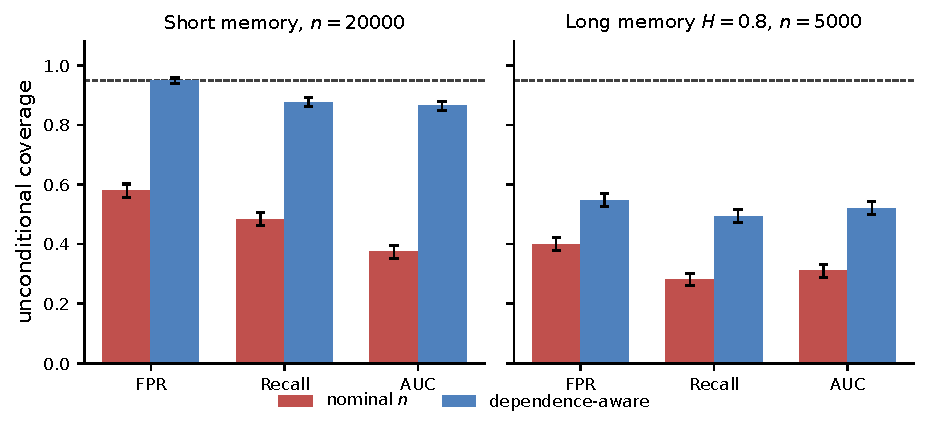
\includegraphics[width=\textwidth]{figures/fig_coverage.pdf}
\end{figure*}

\begin{table}[ht]
\centering
\caption{False-positive coverage, threshold-conditional, $n{=}5000$, $R{=}500$. ESS-Wilson replaces
$n$ by $\neff$ inside the Wilson interval. A cell is unconditional coverage $\pm$ Monte Carlo SE.
Parentheses, when present, are (conditional coverage $\pm$ its Monte Carlo SE, computable
fraction). From
\texttt{results/coverage\_sim.csv}.}\label{tab:covfpr}
\onetab
%
% cell = unconditional coverage $\pm$ Monte Carlo SE; parenthesis = (conditional coverage $\pm$ its Monte Carlo SE, computable fraction) when that fraction is below 0.995
\begin{tabular*}{\tabwidth}{@{\extracolsep{\fill}}lccc@{}}
\toprule
scenario & naive Wilson & ESS-Wilson & \cellbr{moving}{block}\\
\midrule
iid (control) & $0.95\pm0.01$ & $0.95\pm0.01$ & $0.95\pm0.01$ \\
campaigns only & $0.96\pm0.01$ & $0.96\pm0.01$ & $0.92\pm0.01$ \\
background only & $0.60\pm0.02$ & $0.93\pm0.01$ & $0.86\pm0.02$ \\
both & $0.59\pm0.02$ & $0.92\pm0.01$ & $0.87\pm0.01$ \\
long-range ($H{=}0.8$) & $0.40\pm0.02$ & $0.55\pm0.02$ & $0.60\pm0.02$ \\
\bottomrule
\end{tabular*}

\end{table}

\begin{table*}[!t]
\centering
\caption{Recall coverage, same run and cell format as Table~\ref{tab:covfpr}. The ESS plug-in is
the interval on attack indicators after benign gaps are removed. The episode bootstrap is a
different procedure.}\label{tab:covrec}
\fulltab
%
% cell = unconditional coverage $\pm$ Monte Carlo SE; parenthesis = (conditional coverage $\pm$ its Monte Carlo SE, computable fraction) when that fraction is below 0.995
\begin{tabular*}{\tabwidth}{@{\extracolsep{\fill}}lcccc@{}}
\toprule
scenario & \cellbr{naive}{normal} & \cellbr{ESS}{plug-in} & \cellbr{episode}{bootstrap} & \cellbr{moving}{block}\\
\midrule
iid (control) & $0.95\pm0.01$ & $0.95\pm0.01$ & $0.94\pm0.01$ & $0.94\pm0.01$ \\
campaigns only & \cellbr{$0.70\pm0.02$}{$(0.95\pm0.01,\,0.74)$} & \cellbr{$0.70\pm0.02$}{$(0.95\pm0.01,\,0.74)$} & \cellbr{$0.24\pm0.02$}{$(0.32\pm0.02,\,0.74)$} & \cellbr{$0.61\pm0.02$}{$(0.82\pm0.02,\,0.74)$} \\
background only & $0.87\pm0.01$ & $0.93\pm0.01$ & $0.85\pm0.02$ & $0.88\pm0.01$ \\
both & \cellbr{$0.32\pm0.02$}{$(0.45\pm0.03,\,0.72)$} & \cellbr{$0.54\pm0.02$}{$(0.76\pm0.02,\,0.72)$} & \cellbr{$0.22\pm0.02$}{$(0.30\pm0.02,\,0.73)$} & \cellbr{$0.47\pm0.02$}{$(0.65\pm0.03,\,0.73)$} \\
long-range ($H{=}0.8$) & \cellbr{$0.28\pm0.02$}{$(0.38\pm0.03,\,0.74)$} & \cellbr{$0.49\pm0.02$}{$(0.67\pm0.02,\,0.73)$} & \cellbr{$0.20\pm0.02$}{$(0.27\pm0.02,\,0.74)$} & \cellbr{$0.46\pm0.02$}{$(0.62\pm0.03,\,0.74)$} \\
\bottomrule
\end{tabular*}

\end{table*}

\begin{table*}[!t]
\centering
\caption{AUC coverage, same run and cell format. The moving-block column resamples label and
score jointly inside each temporal block, so their local association is kept; positive and negative
scores are not drawn as two independent samples. There is no ESS plug-in for the
AUC.}\label{tab:covauc}
\fulltab
%
% cell = unconditional coverage $\pm$ Monte Carlo SE; parenthesis = (conditional coverage $\pm$ its Monte Carlo SE, computable fraction) when that fraction is below 0.995
\begin{tabular*}{\tabwidth}{@{\extracolsep{\fill}}lccc@{}}
\toprule
scenario & \cellbr{i.i.d.}{bootstrap} & \cellbr{moving}{block} & \cellbr{block}{jackknife}\\
\midrule
iid (control) & $0.93\pm0.01$ & $0.92\pm0.01$ & $0.93\pm0.01$ \\
campaigns only & \cellbr{$0.69\pm0.02$}{$(0.93\pm0.01,\,0.74)$} & \cellbr{$0.61\pm0.02$}{$(0.83\pm0.02,\,0.74)$} & \cellbr{$0.55\pm0.02$}{$(0.74\pm0.02,\,0.74)$} \\
background only & $0.91\pm0.01$ & $0.93\pm0.01$ & $0.93\pm0.01$ \\
both & \cellbr{$0.26\pm0.02$}{$(0.36\pm0.03,\,0.73)$} & \cellbr{$0.56\pm0.02$}{$(0.78\pm0.02,\,0.73)$} & \cellbr{$0.54\pm0.02$}{$(0.74\pm0.02,\,0.73)$} \\
long-range ($H{=}0.8$) & \cellbr{$0.31\pm0.02$}{$(0.42\pm0.03,\,0.74)$} & \cellbr{$0.52\pm0.02$}{$(0.70\pm0.02,\,0.74)$} & \cellbr{$0.54\pm0.02$}{$(0.72\pm0.02,\,0.74)$} \\
\bottomrule
\end{tabular*}

\end{table*}

\begin{table*}[!t]
\centering
\caption{The factorial at $n{=}20000$, $R{=}500$. The episode bootstrap and long memory were not rerun at this $n$. From
\texttt{results/coverage\_sim\_n20000.csv}.}\label{tab:covn}
\fulltab
%
% cell = unconditional coverage $\pm$ Monte Carlo SE; parenthesis = (conditional coverage $\pm$ its Monte Carlo SE, computable fraction) when that fraction is below 0.995
\begin{tabular*}{\tabwidth}{@{\extracolsep{\fill}}lcccccc@{}}
\toprule
scenario & \cellbr{FPR}{naive} & \cellbr{FPR}{ESS-Wilson} & \cellbr{recall}{naive} & \cellbr{recall}{ESS} & \cellbr{AUC}{i.i.d.} & \cellbr{AUC}{block}\\
\midrule
iid (control) & $0.96\pm0.01$ & $0.96\pm0.01$ & $0.95\pm0.01$ & $0.96\pm0.01$ & $0.93\pm0.01$ & $0.93\pm0.01$ \\
campaigns only & $0.95\pm0.01$ & $0.95\pm0.01$ & \cellbr{$0.95\pm0.01$}{$(0.95\pm0.01,\,0.99)$} & \cellbr{$0.95\pm0.01$}{$(0.96\pm0.01,\,0.99)$} & \cellbr{$0.91\pm0.01$}{$(0.92\pm0.01,\,0.99)$} & \cellbr{$0.89\pm0.01$}{$(0.90\pm0.01,\,0.99)$} \\
background only & $0.56\pm0.02$ & $0.94\pm0.01$ & $0.91\pm0.01$ & $0.95\pm0.01$ & $0.92\pm0.01$ & $0.95\pm0.01$ \\
both & $0.58\pm0.02$ & $0.95\pm0.01$ & $0.48\pm0.02$ & $0.88\pm0.01$ & $0.37\pm0.02$ & $0.86\pm0.01$ \\
\bottomrule
\end{tabular*}

\end{table*}

\subsection{Where the short-memory procedure stops working}\label{sec:hurst}
A single Hurst value shows that a short-memory procedure can fail. It does not say where. Holding
the long-memory cell's generator, threshold rule, $n$, $R$, $B$ and seed fixed and varying $H$ alone
gives Table~\ref{tab:hurst}. The $H{=}0.8$ arm reproduces the row in Table~\ref{tab:covfpr} by
construction, which is what makes the rest of the column comparable to it.

Three things are visible in Figure~\ref{fig:hurst}. First, the plug-in has a usable region: at $H{=}\HGridLo$ and $H{=}0.6$
ESS--Wilson covers at $\FprHLo$ and $\FprHSix$, so the procedure is not merely a short-memory
artefact of the AR(1) cells. Second, the degradation is monotone and steep rather than a cliff:
$\FprHSeven$ at $H{=}0.7$, $\FprLrdEss$ at $H{=}0.8$, $\FprHNine$ at $H{=}\HGridHi$. Third, the
ordering of the two constructions reverses inside the grid. At $H{=}0.7$ the plug-in is still ahead
of the moving block ($\FprHSeven$ against $\FprHSevenMbb$); by $H{=}0.8$ the moving block is ahead
($\FprHEightMbb$ against $\FprLrdEss$), and it stays ahead at $H{=}\HGridHi$. Neither reaches
nominal once $H\ge0.7$, so the reversal is a ranking between two failing procedures, not a
recommendation.

The mechanism is the one the theory predicts, and the instrument reports it without being asked.
For $H>1/2$ the autocovariances of fractional Gaussian noise need not be summable, so
$\tau_{\mathrm{int}}$ has no finite limit to estimate; what a truncation rule returns instead grows
with the dependence. The mean Geyer estimate on the score series rises across the grid and the mean
$\neff$ falls from $\NeffHLo$ at $H{=}\HGridLo$ to $\NeffHNine$ at $H{=}\HGridHi$
(Table~\ref{tab:hurst}). That is a diagnostic a practitioner already has: the same $\neff$ the
reporting line asks for is the quantity that collapses in the regime where the interval built from
it should not be trusted. It is an association across five cells of one generator, not a test with a
calibrated size, and $\neff$ does not separate long memory from a short-memory series with a large
$\tau_{\mathrm{int}}$. The estimator-agreement rule of \S\ref{sec:instrument} is the check that
carries that load, and whether it fires is Table~\ref{tab:gate}.

It does not fire, if it is applied where the interval takes its $\neff$ from
(Figure~\ref{fig:hurst}, right). Run on the benign
alarm indicator, the gate --- Geyer and batch means within $2\times$, $\neff\ge50$ --- admits
$\GateAlarmEight$ of replicates at $H{=}0.8$ and $\GateAlarmNine$ at $H{=}\HGridHi$, where
ESS--Wilson covers $\FprLrdEss$ and $\FprHNine$. A gate that admits nine replicates in ten while
the interval it admits covers a third of the time is not a safeguard. The reason is visible in the
same table: thresholding at a one-percent rate discards most of the score's serial structure, so the
indicator's $\hat\tau$ is $\TauAlarmNine$ at $H{=}\HGridHi$ where the benign score's is
$\TauScoreNine$. A long-memory score produces a short-memory-looking indicator, and the two
estimators agree with each other about the wrong series.

Run on the benign score series instead, the same rule tracks coverage. It admits every replicate at
$H\le0.6$ ($\GateScoreSix$), where the interval covers $\FprHSix$ or better; $\GateScoreSeven$ at $H{=}0.7$;
$\GateScoreEight$ at $H{=}0.8$; and $\GateScoreNine$ at $H{=}\HGridHi$. The discriminating
quantity is the disagreement, not the floor: the $\neff\ge50$ condition alone admits the score
series in $\GateScoreNeffOnlyNine$ of replicates even at $H{=}\HGridHi$, because $\neff$ there is
still about $\NeffHNine$. This is one family and $R{=}\GateR$ replicates per cell, and it is a screen rather
than a test with a calibrated size --- a short-memory series with a genuinely large
$\tau_{\mathrm{int}}$ can fail it. It is also the reason the reporting rule in
Table~\ref{tab:rule} is stated on the score series: an analyst cannot observe $H$, and the
indicator they are about to build the interval from is the one series that will not warn them.
\begin{table*}[!t]
\centering
\caption{Whether the reporting gate detects the regime in which its own interval fails. The gate is
Geyer and batch means within $2\times$ and $\neff\ge50$; ``admits'' is the fraction of $R{=}\GateR$
replicates it passes. Applied to the alarm indicator it admits almost everything; applied to the
benign score series that generates those alarms it tracks coverage. $\hat\tau$ entries are medians.
Coverage is the ESS--Wilson column of Table~\ref{tab:hurst}. From
\texttt{diagnostics/}\allowbreak\texttt{p127\_gate.csv}.}\label{tab:gate}
\fulltab
\begin{tabular*}{\tabwidth}{@{\extracolsep{\fill}}llcccc@{}}
\toprule
$H$ & \cellbr{ESS-Wilson}{coverage} & \cellbr{alarm indicator}{$\hat\tau$ Geyer / batch} & \cellbr{gate admits}{(indicator)} & \cellbr{benign score}{$\hat\tau$ Geyer / batch} & \cellbr{gate admits}{(score)}\\
\midrule
0.55 & $0.96\pm0.01$ & 1.03 / 1.04 & 1.00 & 1.4 / 1.5 & 1.00 \\
0.6 & $0.93\pm0.01$ & 1.07 / 1.10 & 1.00 & 2.2 / 2.3 & 1.00 \\
0.7 & $0.82\pm0.02$ & 1.24 / 1.39 & 1.00 & 6.8 / 5.1 & 0.89 \\
0.8 & $0.55\pm0.02$ & 1.78 / 2.05 & 0.99 & 23.9 / 10.9 & 0.40 \\
0.9 & $0.33\pm0.02$ & 3.62 / 3.56 & 0.92 & 74.2 / 20.8 & 0.11 \\
\bottomrule
\end{tabular*}
% source diagnostics/p127_gate_vs_memory.py -> diagnostics/p127_gate.csv; coverage from results/hurst_sweep.csv

\end{table*}
\begin{figure*}[!t]
\centering
\caption{Left: unconditional false-positive coverage against the Hurst exponent, for the
nominal-$n$ interval, the ESS--Wilson plug-in and the moving-block bootstrap. Error bars are Monte
Carlo standard errors; the dashed line is the nominal $0.95$. Right: the fraction of replicates the
prespecified gate admits --- Geyer and batch means within $2\times$ and $\neff\ge50$ --- computed on
the alarm indicator the interval is built from and on the benign score series behind it, against
the same coverage curve. The indicator gate stays near one while coverage falls to $\FprHNine$.
$n{=}5000$, $R{=}500$. From \texttt{results/hurst\_sweep.csv} and
\texttt{diagnostics/p127\_gate.csv}.}\label{fig:hurst}
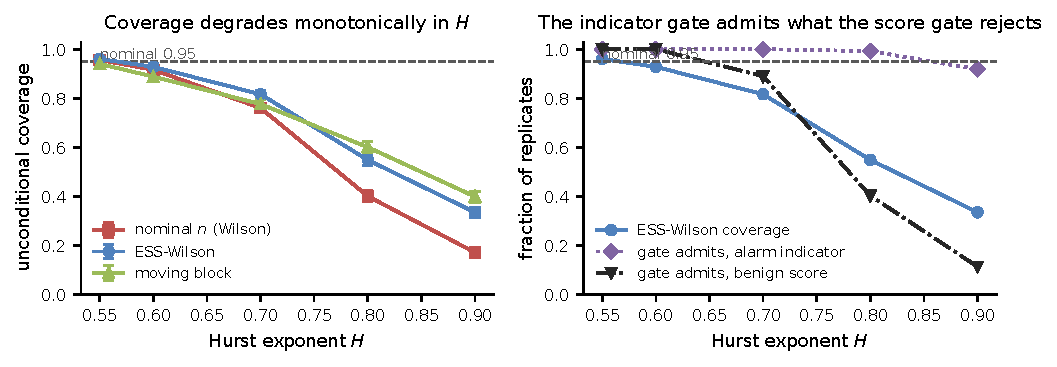
\includegraphics[width=\textwidth]{figures/fig_hurst.pdf}
\end{figure*}

\begin{table*}[!t]
\centering
\caption{Coverage against the Hurst exponent. Fractional-Gaussian background, campaign labels,
$n{=}5000$, $R{=}500$, $B{=}200$, seed $0$; only $H$ varies. $\star$ marks the value reported in
Tables~\ref{tab:covfpr}--\ref{tab:covauc}, which this run reproduces. $\neff$ is the mean Geyer
effective sample size of the benign score series, the quantity the reporting line asks for. Cells
are unconditional coverage $\pm$ Monte Carlo SE. From
\texttt{results/hurst\_sweep.csv}.}\label{tab:hurst}
\fulltab
\begin{tabular*}{\tabwidth}{@{\extracolsep{\fill}}llccccc@{}}
\toprule
$H$ & \cellbr{mean $\neff$}{(score series)} & \cellbr{FPR}{naive Wilson} & \cellbr{FPR}{ESS-Wilson} & \cellbr{FPR}{moving block} & \cellbr{recall}{ESS} & \cellbr{AUC}{moving block}\\
\midrule
0.55 & 1087 & $0.96\pm0.01$ & $0.96\pm0.01$ & $0.94\pm0.01$ & $0.75\pm0.02$ & $0.65\pm0.02$ \\
0.6 & 853 & $0.92\pm0.01$ & $0.93\pm0.01$ & $0.89\pm0.01$ & $0.68\pm0.02$ & $0.62\pm0.02$ \\
0.7 & 365 & $0.76\pm0.02$ & $0.82\pm0.02$ & $0.78\pm0.02$ & $0.58\pm0.02$ & $0.59\pm0.02$ \\
0.8$\star$ & 145 & $0.40\pm0.02$ & $0.55\pm0.02$ & $0.60\pm0.02$ & $0.49\pm0.02$ & $0.52\pm0.02$ \\
0.9 & 64 & $0.17\pm0.02$ & $0.33\pm0.02$ & $0.40\pm0.02$ & $0.36\pm0.02$ & $0.45\pm0.02$ \\
\bottomrule
\end{tabular*}
% source scripts/hurst_sweep.py -> results/hurst_sweep.csv; $\star$ = the H reported in Table~\ref{tab:covfpr}

\end{table*}

\subsection{Order available to the interval}\label{sec:split}
For the stationary generator used here, the random partition preserves the marginal
point-estimation target, while changing which temporal neighbours remain in the test subset. If
that sequence is then analysed
in shuffled order, the estimator of $\tau_{\mathrm{int}}$ cannot see the dependence that remains.

Table~\ref{tab:split} is one run of the false-positive interval on the short-memory campaign
generator ($n{=}20000$, $R{=}500$). On the time-ordered test half, naive Wilson coverage is
$\SplitTempNaive$ and ESS-Wilson coverage is $\SplitTempEss$, at $\tau_{\mathrm{int}}{=}\TauTemp$. On the
shuffled test sequence the two intervals cover at $\SplitShuf$ and $\SplitShufEss$, and the
autocorrelation time in that order is $\TauShuf$. On the same random partitions, with the test
indices sorted back into original time before the interval is built, naive coverage stays
$\SplitRestNaive$ and ESS-Wilson coverage rises to $\SplitRestEss$, at
$\tau_{\mathrm{int}}{=}\TauRest$. These $\tau$ values are those of the benign score series, which
is what the order experiment manipulates. They are not the divisor the interval applies: ESS-Wilson
takes $\neff$ from the alarm indicator, whose autocorrelation time is smaller because thresholding
discards most of the score's serial structure. That gap is benign here and is not benign under long
memory, where it is what stops the quality gate from firing (\S\ref{sec:hurst}). The order presented to the estimator
determines whether it detects the serial structure. The third row keeps the random-partition subset
and restores only its original temporal order, so $\tau_{\mathrm{int}}{=}\TauRest$ is the dependence
among that subset. It is not the time-ordered half's $\TauTemp$, and the row is not expected to
reproduce the first. A release whose timestamps are dropped or colliding cannot be reconstructed
from the released sequence alone.
\begin{table}[ht]
\centering
\caption{False-positive coverage by the order the interval is allowed to see. ESS-Wilson is the
plug-in of \S\ref{sec:instrument}. The third row preserves the random-partition subset and restores
only its original temporal ordering; it is therefore not expected to reproduce the time-ordered
test-half $\tau$. $\tau$ is the mean Geyer autocorrelation time of the benign \emph{scores} in the
order the interval saw; the ESS-Wilson divisor is the alarm indicator's, which is smaller.
$n{=}20000$, $R{=}500$, seed 1. From
\texttt{results/split\_order\_arms.csv}.}\label{tab:split}
\onetab
\begin{tabular*}{\tabwidth}{@{\extracolsep{\fill}}lccc@{}}
\toprule
\cellbr{order available}{to the interval} & \cellbr{naive}{Wilson} & ESS-Wilson & \cellbr{$\tau$ in}{that order}\\
\midrule
\cellbr{time-ordered}{test half} & $0.60\pm0.02$ & $0.95\pm0.01$ & 19.5 \\
\cellbr{shuffled}{test sequence} & $0.71\pm0.02$ & $0.71\pm0.02$ & 1.0 \\
\cellbr{same partition,}{time restored} & $0.71\pm0.02$ & $0.94\pm0.01$ & 10.2 \\
\bottomrule
\end{tabular*}
% tau seen: temporal 19.51, shuffled 1.02, same points in true time 10.2; n=20000, R=500, seed=1

\end{table}

\subsection{Feature-level dependence in telemetry}\label{sec:dif}
We measure feature-level estimated $\DIF$ on time-order-audited telemetry at three grains. These
are recorded series, not alarm indicators. The real-data analysis provides evidence of serial
dependence in the series that pass the filter, and it shows heterogeneity across features and
windows. Alarm-indicator intervals are \S\ref{sec:metric}, and coverage on a resampled Monday
prefix is Table~\ref{tab:rule}. The headline figures are
QC-filtered descriptive estimates: a series enters only when it is not a deterministic function of
the index, Geyer and batch means agree within a factor of two, and $\neff\ge50$. The packet value
near $\PktQGeyer$ and the window median near $\WinQMed$ are medians of the series that pass. They are not an
estimate of the dependence distribution over every feature in the capture. Time order is verified before
any estimate: a dataset with non-monotone or colliding timestamps, or shipped without a timestamp,
cannot have its dependence reconstructed from the released sequence alone. A single estimated
autocorrelation time describes a series only where that dependence is stable enough to be
summarised by one number. The flow byte-rate below is the counterexample.

\paragraph{Packet grain} From the CICIDS2017 capture in true sub-second order (pcapng), across
three non-adjacent windows spanning about five hours (Table~\ref{tab:packet}), only the early
inter-arrival window qualifies under the estimator-agreement QC rule (Geyer $\PktQGeyer$, batch
$\PktQBatch$, $\neff\!=\!\PktQNeff$): one series, not a median across windows, with
$\DIF\!\approx\!2$. In the mid and late windows Geyer and batch means diverge sharply
($\PktMidGeyer$ vs $\PktMidBatch$; $\PktLateGeyer$ vs $\PktLateBatch$). A
block length of twice the estimated autocorrelation time would differ by that same factor, which is
why those windows are reported as disagreement between the two estimators, spanning $\PktRangeLo$
to $\PktRangeHi$, and not as the spread of one estimator or as a point used to set $L$. The per-second series fails
the reporting floor ($\neff\!<\!50$) and packet size is flagged. The qualifying estimate is the early
window, near $2$. The mid and late windows are the non-qualifying disagreement.
\begin{table*}[!t]
\centering
\caption{Packet-grain $\DIF$, three non-adjacent CICIDS2017 windows (true pcapng order), with window
length, $\neff$ and agreement-rule status. From \texttt{results/packet\_windows.csv}.}\label{tab:packet}
\fulltab
\begin{tabular*}{\tabwidth}{@{\extracolsep{\fill}}lllccl@{}}
\toprule
window & len (s) & series & \cellbr{DIF}{(geyer/batch)} & $n_{\mathrm{eff}}$ & rule\\
\midrule
early & 21 & inter\_arrival & 2.1/1.8 & 43576 & qualifies \\
early & 21 & packets\_per\_1s & 1/1 & 22 & not est. \\
mid & 203 & inter\_arrival & 163.4/26.9 & 481 & est.\ range \\
mid & 203 & packet\_size & 1505/52.3 & 52 & est.\ range \\
late & 128 & inter\_arrival & 152/16.5 & 190 & est.\ range \\
\bottomrule
\end{tabular*}

\end{table*}


\paragraph{Flow grain} On CICIDS2017 flows the shipped timestamp is minute-resolution.
Engelen, Rimmer and Joosen, and Lanvin and colleagues, document flow-construction, labelling,
timestamp, and packet-order defects in this
release~\citep{engelen2021troubleshooting,lanvin2023cicids}; the series below are the as-shipped flows, not a
repaired reconstruction. Duration, byte rate, and inter-arrival time are CICFlowMeter time
features~\citep{lashkari2017tor}. We report
a within-minute-order sensitivity estimate (b) as the primary column and show the as-shipped row-order value (a)
alongside it (Table~\ref{tab:flowdif}); (a) is not a bound on (b): for several features the shuffle
estimate exceeds the as-shipped value, so the as-shipped order bounds the dependence neither per cell
nor at the median. The observed dependence is consistent with serial dependence: within-minute
shuffling does not collapse it, and deduplicating five-tuples does not either. It is feature- and
capture-dependent: the flow byte-rate is
near $\FlowBpsMon$ on Monday and Tuesday and $\FlowBpsWed$ on Wednesday
(Table~\ref{tab:flowdif}). That day-to-day
change is a boundary on the single-$\tau_{\mathrm{int}}$ summary: one global autocorrelation time
does not describe this capture. Sub-minute order is not identified by a minute timestamp: the
shuffle is a sensitivity analysis, and no within-day estimate was computed. These are different
summaries from the qualifying as-shipped flow median $\FlowQualMed$ in Table~\ref{tab:grain}.
The within-minute-shuffle median over features is $\FlowShuffleMed$. Neither number is a DIF for the capture.
\begin{table}[ht]
\centering
\caption{CICIDS2017 benign flow-grain $\DIF$, three days. Each entry is the within-minute-shuffle
estimate, with the as-shipped value in parentheses; that value is not a bound. From
\texttt{results/cicids\_flow\_dif.csv}.}\label{tab:flowdif}
\onetab
\begin{tabular*}{\tabwidth}{@{\extracolsep{\fill}}>{\raggedright\arraybackslash}p{2.35cm}ccc@{}}
\toprule
benign feature & Mon & Tue & Wed\\
\midrule
Bwd Packet Length Mean & 38.6 (45) & 17.5 (14) & 15.3 (17) \\
Flow Bytes/s & 1.0 (1) & 1.0 (1) & 64.0 (63) \\
Flow Duration & 28.2 (44) & 12.2 (61) & 38.2 (63) \\
Flow IAT Mean & 18.1 (12) & 8.2 (6) & 20.5 (17) \\
Flow Packets/s & 5.7 (6) & 10.5 (6) & 31.6 (26) \\
\bottomrule
\end{tabular*}

\end{table}


\paragraph{Window grain (corroboration)} On our own AAL MQTT-bridge telemetry, whose time order we
control and can defend in full, most benign window features fail the QC rule ($\neff\!<\!50$
or Geyer/batch divergence) and two clock encodings (\texttt{time\_sin}, \texttt{time\_cos}) are
excluded as deterministic functions of the index; on the $\WinQn$ qualifying, non-deterministic features
the window-grain $\DIF$ has median $\WinQMed$ (the all-feature median, $\WinAllMed$, is dominated by flagged
series and is reported only beside it). This is corroboration, not the anchor: at $\WinQMed$ it is
still above the $\DIF\!=\!2$ line, consistent with the public-benchmark grains. The series is built
from MQTT alert-stream telemetry we captured from an ambient-assisted-living deployment (benign
windows) with attack windows injected through an isolated-broker testbed, aggregated at a
$60$-minute window grain in native acquisition order; no third-party recording is replayed into it.
\begin{table}[ht]
\centering
\caption{Benign-stream $\DIF$ by grain under the agreement rule (non-deterministic, Geyer and batch
means within $2\times$, $\neff\ge50$). The qualifying entry is the
median of the series that pass; with one packet series that entry is the series itself. From
\texttt{results/dif\_headline.csv}.}\label{tab:grain}
\onetab
\begin{tabular*}{\tabwidth}{@{\extracolsep{\fill}}>{\raggedright\arraybackslash}p{2.2cm}cc>{\raggedright\arraybackslash}p{2.15cm}@{}}
\toprule
 grain (dataset) & \cellbr{qualifying}{DIF ($n$)} & \cellbr{all-series}{median} & other series\\
\midrule
packet (CICIDS pcap) & 2.1 (1) & 152 & 3 range, 1 not-est. \\
flow (CICIDS as-shipped) & 3.4 (4) & 18 & 11 range, 0 not-est. \\
window (AAL, owned) & 3.5 (3) & 96 & 1 range, 10 not-est., 2 determ. \\
\bottomrule
\end{tabular*}
% The qualifying entry is the median of the qualifying series. n=1 is that single series, not a distributional median.
% flow qualifying is the as-shipped (a) order; the within-minute-shuffle (b) median is 17, Table~\ref{tab:flowdif}

\end{table}

\subsection{A dependence-free estimand mismatch}\label{sec:results-sf1}
Even with no dependence, a naive test-set FPR interval covers the deployment (population) metric at
$\SfOnePop$ while covering the threshold-conditional metric at $\SfOneCond$; the Wilson interval
covers that conditional target at $\SfOneWilson$ (Table~\ref{tab:sf1}). The gap is
threshold-estimation uncertainty propagated into the population metric, $\mathrm{Var}[p(\hat T)]$,
which an interval that conditions on the realized threshold does not include. It is not
$\mathrm{Var}(\hat T)$ in isolation. The threshold rule here is the training-benign quantile at a one-percent false-positive
target. For a detector whose threshold is frozen before the test set is seen, the
threshold-conditional interval is the estimand, and the $\SfOneCond$ coverage is not a defect in
that
interval. The mismatch is reading it as the population metric under a re-learned threshold.
\begin{table}[ht]
\centering
\caption{The conflation gap under independence. From
\texttt{diagnostics/p1\_estimand.py}.}\label{tab:sf1}
\onetab
\begin{tabular*}{\tabwidth}{@{\extracolsep{\fill}}llc@{}}
\toprule
interval & estimand & coverage\\
\midrule
naive-normal FPR & population (deployment) & 0.83\\
naive-normal FPR & threshold-conditional & 0.93\\
Wilson FPR & threshold-conditional & 0.95\\
\bottomrule
\end{tabular*}
% source: diagnostics/p1_estimand.py -> diagnostics/p1_iid.csv, iid, R=1000

\end{table}

\subsection{Reported uncertainty in an illustrative sample}\label{sec:results-sf2}
Two nested populations are reported here and they are not interchangeable.
The \emph{SF-2 coding set} is every screened record coded for which estimand its reported uncertainty targets, whether or not its split was time-aware: \NsfTwoRes{} of \NsfTwo{} resolved far enough to code, \NsfTwoStrict{} of them from fetched full text or arXiv source, and \NsfTwoUnres{} did not resolve and are carried as unknown.
The \emph{in-frame pool} is the narrower frame of the retired prevalence hypothesis, which additionally requires a time-aware split \emph{and} a reported interval: \NinframeRes{} of \Ninframe{} records (\ResRate\%) resolved, which is why no prevalence is claimed (\S\ref{sec:limitations}).
Table~\ref{tab:sf2} is the uncertainty kind on the SF-2 coding set, not on the in-frame pool: most report none, and seed or fold dispersion outnumbers a test-set interval \NsfTwoSeedFold{} to \NsfTwoTestCI{}.
\begin{table}[H]
\centering
\caption{Uncertainty kind in the SF-2 coding set ($\NsfTwoRes$ of $\NsfTwo$ screened records
resolved far enough to code). This is the wider of the two populations of
\S\ref{sec:results-sf2}: it does not require a time-aware split, so it is not the \Ninframe-record
in-frame pool. Unresolved records are reported as unknown, never as none.
From \texttt{corpus/sf2\_uncertainty\_kind.csv}.}\label{tab:sf2}
\onetab
\begin{tabular*}{\tabwidth}{@{\extracolsep{\fill}}lcc@{}}
\toprule
uncertainty kind & \cellbr{strict fetched}{($n{=}18$)} & \cellbr{resolved}{($n{=}20$)}\\
\midrule
none (point estimates) & 13 & 15\\
seed-dispersion & 2 & 2\\
fold-dispersion & 1 & 1\\
test-set CI/SE/test & 2 & 2\\
\midrule
\multicolumn{3}{@{}p{\linewidth}@{}}{unresolved (UNKNOWN, not coded none): 11}\\
\bottomrule
\end{tabular*}

\end{table}
These are frequencies in that sample. They are not a prevalence.
Seed or fold dispersion is model-fitting instability on a fixed test set, and its standard error shrinks as the seed count rises (Table~\ref{tab:sf2sim}, Appendix~\ref{app:seed}).
Among the records resolved in the SF-2 coding set, none described a time-aware split; that adoption fact is attributed to larger corpora~\citep{arp2022dos,pendlebury2019tesseract,lew2026deployment}.
Several benchmarks are consumed from releases whose timestamps are dropped or colliding, so the dependence cannot be reconstructed from the released sequence alone.

\subsection{Metric-level intervals on the captures}\label{sec:metric}
The tables above estimate feature series. Here the series is the detector.
A temporal split learns the training-benign quantile at a one-percent false-positive target.
On the Monday prefix, which contains no attacks, the isolation-forest~\citep{liu2008isolation} false-positive interval is wider than the nominal-$n$ interval by a factor $\MonIfFprRatio$, at $\DIF=\MonIfFprDif$.
Wednesday's isolation-forest alarm indicator is a different series, with $\DIF=\WedIfFprDif$, and it is not the Monday result.
Figure~\ref{fig:decision} shows that prefix beside Wednesday and the three Wednesday detector pairs.
The logistic-regression minus random-forest~\citep{breiman2001random} AUC difference is $\WedAucFlip$.
The i.i.d.\ interval excludes zero and the moving-block interval includes zero.
DeLong's covariance for that contrast assumes independent cases~\citep{delong1988comparing}.
The clustered AUC adjustment still assumes exchangeable groups and has no serial dependence
time~\citep{bay2023dependency}.
The $0$--$1$ loss difference for that pair excludes zero under both intervals.
The larger gaps on Tuesday and Wednesday stay away from zero under both intervals.
The isolation-forest versus random-forest score series on Wednesday fails the estimator-agreement rule; that pair is marked in the figure and is not a qualifying comparison.
\begin{figure*}[!t]
\centering
\caption{Left: false-positive intervals on the benign alarm indicator. Monday is a prefix with no attacks. Right: Wednesday AUC differences for the three detector pairs. The asterisk marks a score series whose Geyer and batch-means estimates disagree. From \texttt{results/metric\_level\_intervals.csv} and \texttt{results/paired\_block\_comparisons.csv}.}\label{fig:decision}
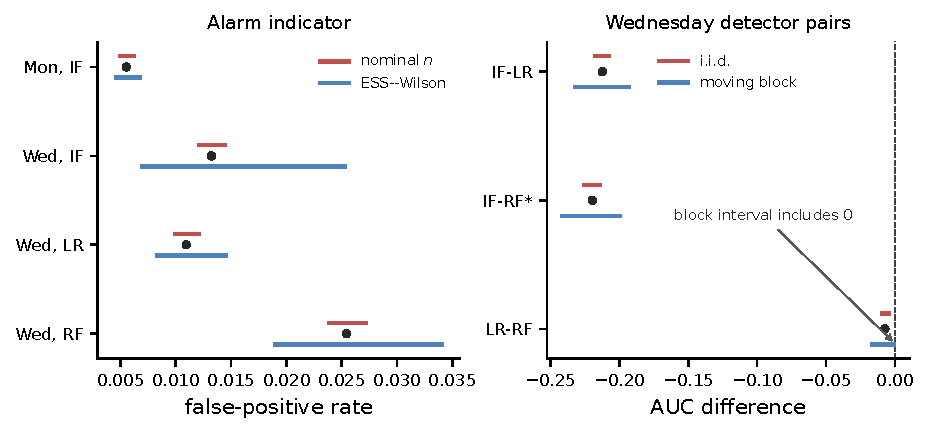
\includegraphics[width=\textwidth]{figures/fig_decision.pdf}
\end{figure*}


\FloatBarrier
\section{Discussion}
\subsection{Simulation and telemetry answer different questions}
The simulation and the telemetry tables answer different questions. In the simulation, metric-level
dependence is the dependence of the series the interval uses, and the result is coverage against a
named target. In the telemetry tables, feature-level dependence is evidence that serial dependence
is present in recorded series. A feature-level $\DIF$ is not the inflation of a false-positive
rate, a recall, or an AUC. The simulation does not establish that the procedures are valid for
dependent IDS telemetry in general. It reports coverage for the generator, the targets, and the
three constructions tested here.

\subsection{Coverage is specific to the metric and the regime}
Where empirical coverage rises, and where it does not, is in \S\ref{sec:coverage}, including the
long-memory grid of \S\ref{sec:hurst} and the campaigns-only AUC drop. The width diagnostics separate the three
constructions further: in the tested cells the false-positive plug-in's variance tracks the
estimator's variability, the recall plug-in's does not once campaigns sit on a dependent
background, and the moving-block resampling distribution is narrower than the sampling
distribution of the AUC. Substituting an effective sample size is not by itself a dependence
correction; the variance construction has to match the stochastic structure of the particular
metric. Nor is a quality gate automatically a safeguard: the series a gate is computed on decides
what it can see, and the thresholded indicator an alarm-rate interval is built from is the series
least able to reveal long memory (\S\ref{sec:hurst}). Higher coverage is not an efficiency result.
The block length is one prespecified rule. These runs do not select it. Flow Bytes/s in
Table~\ref{tab:flowdif} is why one autocorrelation time does not describe that capture.

\subsection{Objections the evidence already answers}
Three objections sit next to evidence already in the paper. The constructions are the block
bootstrap and an ESS plug-in~\citep{kunsch1989jackknife,geyer1992practical}: both are standard, and the contribution is their use on the series
each metric actually uses, with coverage against a named target (\S\ref{sec:instrument},
\S\ref{sec:coverage}). Biostatistics already treats clustered AUC: Bay et al.\ state that their
adjustment does not extend to serial dependence (\S\ref{sec:related}). A time-aware split can
reduce temporal leakage in the point estimate~\citep{arp2022dos,pendlebury2019tesseract}; the time-ordered test half in \S\ref{sec:split} still
has naive false-positive coverage $\SplitTempNaive$. A random partition does not by itself make
the interval uncorrectable: restoring the subset's original order changes the interval
(\S\ref{sec:split}).

\FloatBarrier
\section{Limitations and future work}\label{sec:limitations}
Table~\ref{tab:rule} in \S\ref{sec:objective} is what a reported interval is allowed to say; this section and Appendix~\ref{app:limits} are what bounds it.
A Student-$t$ run with the campaign persistence of the ``both'' cell was scored against \eqref{eq:cond}, so it is not a coverage result and does not appear in Tables~\ref{tab:covfpr}--\ref{tab:covauc}.

On the short-memory campaign generator, the attack-subsequence ESS plug-in and the same plug-in with benign rows left as missing on the original clock are Table~\ref{tab:clock}.
Campaigns are contiguous, so a lag along the attack subsequence and a lag on the original index coincide inside a run.
At $n{=}5000$ the two coverages are $\RecallClockSubFive$ and $\RecallClockMisFive$. At $n{=}20000$ they are $\RecallClockSubTwenty$ and $\RecallClockMisTwenty$.
At both sizes the absolute difference is within two combined Monte Carlo standard errors.
The reported recall interval keeps the subsequence. This comparison uses its own seed. The recall coverage in \S\ref{sec:coverage} remains the coverage-simulation run.
\begin{table}[ht]
\centering
\caption{Recall coverage of two clocks on the same replicates. Short-memory campaign generator, threshold-conditional target, $R{=}500$. Cell format matches Tables~\ref{tab:covfpr}--\ref{tab:covauc}: unconditional coverage, and, when the computable fraction is below 0.995, conditional coverage and that fraction. From \texttt{results/recall\_clock.csv}.}\label{tab:clock}
\onetab
%
% cell = unconditional coverage $\pm$ Monte Carlo SE; parenthesis = (conditional coverage $\pm$ its Monte Carlo SE, computable fraction) when that fraction is below 0.995
\begin{tabular*}{\tabwidth}{@{\extracolsep{\fill}}lcc@{}}
\toprule
$n$ & subsequence & \cellbr{missing on the}{original clock}\\
\midrule
5000 & \cellbr{$0.50\pm0.02$}{$(0.70\pm0.02,\,0.72)$} & \cellbr{$0.50\pm0.02$}{$(0.70\pm0.02,\,0.72)$} \\
20000 & \cellbr{$0.87\pm0.01$}{$(0.88\pm0.01,\,0.99)$} & \cellbr{$0.86\pm0.02$}{$(0.87\pm0.02,\,0.99)$} \\
\bottomrule
\end{tabular*}

\end{table}


Six objections bound what a reader can take from the experiments. The rest of the list is Appendix~\ref{app:limits}.
\begin{enumerate}
\item The corpus is an illustration. Of \Npool{} screened records, \NinframeRes{} of \Ninframe{} in-frame records (\ResRate\%) resolved to full text. No prevalence is claimed.
\item Feature-level $\DIF$ is not metric-level coverage. The Monday alarm-indicator width and the Wednesday ranking are metric-level descriptions. They are not coverage of a detector retrained on each replicate. The Monday Flow Duration coverage is a frozen-threshold resample of that prefix.
\item The long-memory boundary is located in one Gaussian family only. $H$ is swept over
$\HGridN$ values of fractional Gaussian noise (\S\ref{sec:hurst}); no other long-memory process,
and no nonstationary alternative, was tested.
\item Reported moving-block intervals use one prespecified length \eqref{eq:L}. The multiplier is evaluated. It is not a selector.
\item The AUC bootstrap sits short of nominal under independence: $\AucCtrlNaive$ for the i.i.d.\ bootstrap and $\AucCtrlMbb$ for the moving block.
\item Flow Bytes/s is near $\FlowBpsMon$ on Monday and $\FlowBpsWed$ on Wednesday, so one autocorrelation time does not describe that capture.
\end{enumerate}


\FloatBarrier
\section{Conclusion}
We evaluate three dependence-aware interval constructions for false-positive rate, recall, and AUC.
In the cells tested, empirical coverage depends on the metric, the dependence regime, and the
construction. The cells that stay below nominal are part of that result. They are not an unfinished
correction. For the false-positive rate, an ESS-adjusted Wilson plug-in raises
empirical coverage from $\FprNtwNaive$ to $\FprNtwEss$ at $n{=}20000$ in the strongest
short-memory cell, which is approximately nominal. ESS-Wilson holds to $H{=}0.6$ under fractional Gaussian
noise and degrades monotonically above it, to $\FprHNine$ at $H{=}\HGridHi$. The gate that is
supposed to withhold it there has to be read on the benign score series: on the alarm indicator the
interval is built from, thresholding masks the long memory and the gate admits $\GateAlarmNine$ of
replicates at that Hurst value. For recall, an ESS plug-in on the ordered attack-row subsequence increases empirical
coverage and stays short of nominal in the strongest short-memory cell. For the AUC, the
moving-block bootstrap of the Mann--Whitney statistic on joint label-score blocks increases
empirical coverage under that same combined dependence and lowers conditional coverage, from
$\AucCampNaiveCond$ to $\AucCampMbbCond$, in the campaigns-only cell at $n{=}5000$. At
$n{=}20000$ the recall ESS plug-in and the AUC moving-block bootstrap cover at $\RecallNtwEss$ and
$\AucNtwMbb$. Those figures are coverage against the stated targets, including the long-run Monte
Carlo reference for AUC. They are not a comparison of
interval length, and they are not a general validity result. The order presented to the dependence
estimator determines whether the serial structure is visible; restoring the order of a
random-partition subset does not reproduce the time-ordered half. The telemetry tables characterize
feature-level dependence. The Monday Flow Duration result in Table~\ref{tab:rule} is a frozen-threshold resample of one benign prefix, not a detector retrained on each draw. Table~\ref{tab:scope} is the reporting line: the claims the experiments support, and the ones they do not.
\begin{table*}[!t]
\centering
\caption{What the reported experiments establish. Each row is the claim a reader can take from the
corresponding section, not a result beyond it.}\label{tab:scope}
\fulltab
\begin{tabularx}{\textwidth}{@{}>{\raggedright\arraybackslash}X l@{}}
\toprule
claim & in this paper\\
\midrule
A nominal-$n$ interval can undercover when the metric's observations are dependent & tested generators\\
Serial dependence is present in the audited telemetry & descriptive\\
One autocorrelation time describes a capture & no\\
ESS-Wilson reaches approximately nominal FPR coverage in the strongest short-memory cells & yes\\
The recall plug-in reaches nominal coverage under combined dependence & no\\
The moving-block AUC interval reaches nominal coverage under combined dependence & no\\
The tested corrections cover in the $H{=}0.8$ condition & no\\
ESS-Wilson has a located long-memory boundary, at about $H{=}0.6$ in this family & yes\\
The agreement gate on the alarm indicator screens out that regime & no\\
The same gate on the benign score series screens it out in this family & yes\\
That boundary transfers to other long-memory or nonstationary processes & untested\\
The telemetry tables calibrate an interval on a real IDS test set & no\\
The results apply to every IDS dataset & no\\
\bottomrule
\end{tabularx}
\end{table*}


\section*{Author contributions}
\textbf{Soheib Cherih:} conceptualization, methodology, software, validation, formal analysis,
investigation, data curation, writing---original draft, visualization.
\textbf{Sabri Lyazid:} conceptualization, methodology, supervision, writing---review \& editing,
project administration.
\textbf{Okba Kazar:} supervision, writing---review \& editing.

\section*{Funding}
This research received no specific grant from any funding agency in the public, commercial, or
not-for-profit sectors.

\section*{Declaration of competing interest}
The authors declare no competing financial interests or personal relationships that could have
appeared to influence the work reported in this paper.

\section*{Ethics}
The study uses the public CICIDS2017 capture and MQTT alert-stream telemetry collected by the
authors from an ambient-assisted-living deployment. The series analysed here are numeric
window-level aggregates of a broker alert stream at a $60$-minute grain --- counts, rates,
inter-arrival summaries, and scalar entropy and diversity statistics. No message payload, topic
string, device or user identifier, or location value appears in them or in any figure or table in
this paper. Attack windows come from a separate isolated-broker testbed with no live participants.
No intervention was performed on the deployment.

\section*{Data and code availability}
The instrument, the coverage simulation, every table, and the screening log are released as a
reproducible artifact: \texttt{make all} regenerates all tables from \texttt{results/} and rebuilds
this paper. The coverage, episode-curve, threshold-mismatch, and telemetry figures in the prose are
macros written from the result and diagnostic files by the script that writes the tables, so a
number cannot be restated by hand. A build-time check fails if the abstract's
dependence-inflation figures drift from those files, if a macro disagrees with the file it came
from, or if a generated macro stops being used in the text. The block-length sensitivity is
produced by a separate script with its own random stream, and its multiplier-$2$ arm reruns the
reported AUC cells; the build fails if the two disagree by more than twice their combined Monte
Carlo standard error. The Hurst sweep of \S\ref{sec:hurst} is a separate script holding the
reported long-memory cell's seed, $n$, $R$ and $B$ fixed, and the build fails if its $H{=}0.8$ arm
stops reproducing that cell, if coverage or $\neff$ stops being monotone in $H$, or if the gate
orderings the reporting rule rests on stop holding. The artifact is
released as a single snapshot of the submitted state. The instrument was frozen before any
real-data analysis and the pre-registration before the corpus was coded; both freezes, and every
subsequent deviation, are dated in \texttt{prereg/CHANGELOG.md}, which ships with the artifact. The
pre-registration, its change log, the verbatim screening criteria, and the full inclusion log
(Option A, single-coder) are in that snapshot. A public archive DOI is not attached to this draft.
The AAL MQTT-bridge window features underlying the window-grain results are available from the
corresponding author on reasonable request; the raw MQTT alert stream is not redistributed, having
been captured from a live deployment. The retired H3a claim-coding arm is not part of the release:
its schema is kept as a record in \texttt{docs/h3a\_schema.md}, and the reason it was retired is
in the pre-registration change log. No claim in this paper depends on it.

\section*{Declaration of generative AI and AI-assisted technologies}
The authors used generative AI and AI-assisted tools during the preparation of this work. After
using these tools, the authors reviewed and edited the content as needed and take full
responsibility for the content of the publication. All quantitative results are regenerated by the
released code and were checked by the authors. Generative AI is not listed as an author.

\appendix
\section{Extended limitations}\label{app:limits}
These are the objections behind Table~\ref{tab:rule}. They constrain the claims. They are not a
second results section. They are grouped by what they limit: the corpus, the telemetry estimates,
the resampling, and the generator.

\paragraph{The corpus}
\begin{enumerate}
\item \textbf{It is illustrative, $n$ is small, and it has two denominators.} The SF-2 coding set
  resolved \NsfTwoRes{} of \NsfTwo{} screened records, and the \NsfTwoUnres{} that did not are
  carried as unknown, never as ``none''. The narrower in-frame pool, which also requires a
  time-aware split and a reported interval, resolved \NinframeRes{} of \Ninframe{} (\ResRate\%).
  The remainder are access-blocked. Table~\ref{tab:sf2} is the first population, and no prevalence
  or survival fraction is claimed on either.
\item \textbf{Single-coder, method-limited enumeration.} No eligible independent coder was
  available, so no $\kappa$ is reported and reproducibility rests on the published log and verbatim
  criteria; the supervisor performed adversarial review of the contested calls. Web-only search
  resolves indexed sources (arXiv, PMC) but not IEEE Xplore or ScienceDirect abstracts, so the
  venue strata are under-enumerated by a method-dependent amount.
\end{enumerate}

\paragraph{The telemetry estimates}
\begin{enumerate}\setcounter{enumi}{2}
\item \textbf{$\DIF$ is itself estimated, and biased low where $\tau_{\mathrm{int}}$ is largest}
  (few effective episodes), so the tables understate dependence in exactly the regimes that matter
  most; this is reported as a directional bias with the Geyer/batch agreement flag. Differential
  $\DIF$ is not estimable at full-day scope ($\neff \approx 40 < 50$); the benign differential is
  $\approx \DiffBenign$, so the paired-test adjustment is small, and the large full-day value is
  not used.
\item \textbf{Resolution and sample-size caveats by grain.} Minute-resolution flow timestamps force
  the within-minute-shuffle estimate; the as-shipped value is a comparator, not a bound --- for
  several features the shuffle estimate exceeds it, so it bounds the dependence neither per cell
  nor at the median. At window grain, after excluding deterministic clock encodings and series
  failing the agreement rule or the $\neff$ floor, \WinQn{} AAL features qualify, so the window
  headline ($\approx\WinQMed$) is corroboration rather than a high-precision estimate.
\item \textbf{Feature-level dependence is not metric-level dependence.} The telemetry tables
  estimate autocorrelation of packet, flow, and window series. The Monday Flow Duration coverage
  in Table~\ref{tab:rule} is a frozen-threshold resample of that benign prefix. It is not a
  detector retrained on each replicate, and it is not coverage for every feature.
\end{enumerate}

\paragraph{The resampling}
\begin{enumerate}\setcounter{enumi}{5}
\item \textbf{The AUC bootstrap under-covers mildly even under independence} ($\approx \AucIid$ in
  the i.i.d.\ control); this is a finite-sample effect of the U-statistic bootstrap that we do not
  fully explain. It is not a small-$B$ artifact: at the pre-registered $B{=}1000$ the control
  coverage is unchanged ($\AucCtrlBhiNaive$/$\AucCtrlBhiMbb$ for naive/MBB, versus
  $\AucCtrlBloNaive$/$\AucCtrlBloMbb$ at $B{=}200$).
\item \textbf{Bootstrap replicates below the pre-registered $B$.} Moving-block and jackknife cells
  in Tables~\ref{tab:covfpr}--\ref{tab:covauc} used $B{=}200$ against the pre-registered $B{=}1000$,
  for runtime (deviation logged). A $B{=}1000$ re-run of the factorial at $n{=}5000$ moved no
  moving-block or i.i.d.-bootstrap AUC coverage beyond its combined Monte Carlo SE. The long-memory
  block-jackknife cell moved from $\AucLrdBjk$ to $\AucLrdBjkBhi$, past that SE. The jackknife is
  not a headline interval. ESS-Wilson and the recall ESS plug-in contain no bootstrap, and
  Table~\ref{tab:split} is Wilson only.
\item \textbf{One prespecified block length.} Reported moving-block intervals use \eqref{eq:L}.
  That rule is evaluated; it is not proposed as a selector. Politis--White is implemented and was
  not used for those cells. Table~\ref{tab:blocklen} varies the multiplier over $\{1,2,4\}$ in two
  AUC cells and finds coverage decreasing slowly in $L$; it does not search for an optimal
  multiplier, and no other metric, scenario, or sample size was rerun. In the non-qualifying packet
  windows Geyer and batch means differ by factors of $\PktFactorMid$ and $\PktFactorLate$; those
  windows are not used to set $L$.
\item \textbf{Efficiency is not evaluated.} Tables~\ref{tab:width} and~\ref{tab:aucmech} use width
  diagnostically, to ask whether a reported standard error matches the estimator's variability.
  They are not an efficiency comparison: no procedure is preferred here for producing a shorter
  interval at equal coverage, and a coverage gain can come from a wider interval.
\end{enumerate}

\paragraph{The generator}
\begin{enumerate}\setcounter{enumi}{9}
\item \textbf{Stationarity is assumed, the halves meet, and the generator models dependence rather
  than traffic.} The coverage generator is a stationary AR(1), stationary fractional Gaussian
  noise, or a stationary Markov campaign; Flow Bytes/s is near $\FlowBpsMon$ on Monday,
  $\FlowBpsTue$ on Tuesday and $\FlowBpsWed$ on Wednesday (Table~\ref{tab:flowdif}), so one
  $\tau_{\mathrm{int}}$ does not describe that series across the capture, and no morning,
  afternoon, or rolling estimate was computed. The threshold is learned on the first half and the
  metric computed on the second: conditioning on the realized threshold defines the target, but it
  does not make the two halves probabilistically independent. The Student-$t$ run is omitted from
  the coverage tables because it was scored against \eqref{eq:cond}, not against the $t_3$ tail.
\item \textbf{The long-memory sweep is one family and one axis.} $H$ is varied over $\HGridN$
  values of fractional Gaussian noise with everything else fixed (\S\ref{sec:hurst}); the
  crossover at which the moving block overtakes the plug-in ($\FprHSevenMbb$ against $\FprHSeven$ at
  $H{=}0.7$, $\FprHEightMbb$ against $\FprLrdEss$ at $H{=}0.8$) is read off a five-point grid at one
  $n$ and one prevalence, so it locates the boundary to within a grid step and no more. A
  subsampling rate following $1-H$ is future work. The method as reported is a short-memory
  procedure whose failure is now bracketed rather than exhibited at a point.
\item \textbf{Three references are cited without a full-text read.} Obuchowski (1997) is
  paywalled, and the clustered-AUC seam is therefore attributed to Bay et al.\ (2023), which was
  read in full. The two language-model-evaluation preprints in \S\ref{sec:related} were verified at
  abstract level and are cited only as precedent that the problem arises in other evaluation
  literatures; no number or claim in this paper rests on them. Every other reference was resolved,
  and the verification log ships with the artifact.
\end{enumerate}

\section{Seed dispersion on a fixed test set}\label{app:seed}
On a fixed test set the standard error of a seed mean shrinks as the seed count rises. That quantity is not the sampling uncertainty of the test metric.
\begin{table}[ht]
\centering
\caption{Seed standard error vs.\ true test-set sampling standard deviation, by seed count $K$
(fixed test set). From \texttt{diagnostics/sf2\_seed\_vs\_testset.py}.}\label{tab:sf2sim}
\onetab
\begin{tabular*}{\tabwidth}{@{\extracolsep{\fill}}ccccc@{}}
\toprule
$K$ seeds & seed\_std & seed\_SE & \cellbr{test-set}{sd} & \cellbr{SE/}{test-set}\\
\midrule
2 & 0.0031 & 0.0022 & 0.0034 & 0.64 \\
5 & 0.0036 & 0.0016 & 0.0034 & 0.48 \\
10 & 0.0030 & 0.0010 & 0.0034 & 0.28 \\
20 & 0.0033 & 0.0007 & 0.0034 & 0.21 \\
50 & 0.0033 & 0.0005 & 0.0034 & 0.14 \\
100 & 0.0032 & 0.0003 & 0.0034 & 0.09 \\
200 & 0.0033 & 0.0002 & 0.0034 & 0.07 \\
\bottomrule
\end{tabular*}

\end{table}


\section{Reproducible methods specification}
\label{app:methods}
Every setting below is fixed in the released instrument; \texttt{make all}
regenerates all results from it. This appendix records the choices a reader needs to reproduce or port
the instrument; it is not a survey.

\paragraph{Autocorrelation time and $\neff$} The integrated autocorrelation time
$\tau_{\mathrm{int}} = 1 + 2\sum_{k\ge 1}\rho_k$ is estimated by the Geyer initial-positive-sequence
truncation~\citep{geyer1992practical}, which sums the empirical autocorrelations while consecutive
lag pairs remain positive and truncates once a pair turns non-positive; the autocorrelations
themselves are computed by FFT. As an independent estimator we also compute $\tau_{\mathrm{int}}$ by
non-overlapping batch means~\citep{flegal2010batch}. The two are reported together with an
agreement flag. The floor guard of \S\ref{sec:instrument} is a heuristic disagreement rule, not a
test that the timestamps are wrong. The effective sample size is $\neff = n/\tau_{\mathrm{int}}$~\citep{geyer1992practical,vehtari2021ess} and the dependence-inflation
factor is $\DIF = n/\neff = \tau_{\mathrm{int}}$.

\paragraph{Block-length selection} Every reported moving-block and block-jackknife interval uses
\eqref{eq:L}: twice the larger of $\hat\tau_y$ and $\hat\tau_s$, at least $2$, and at most
$\lfloor n^{2/3}\rfloor$. A Politis--White selector~\citep{politis2004automatic,patton2009correction} is implemented in
\texttt{politis\_white\_block\_length} and was not the length used for any coverage number here.
Under weak dependence the mean-squared-error block length for a variance is of order
$n^{1/3}$~\citep{hall1995blocking}; under long memory, including fractional Gaussian noise, a larger
order is not automatically better~\citep{zhang2022block,lahiri2003resampling}. None of
those results selects the multiplier $2$. Table~\ref{tab:blocklen} reports what multipliers $1$ and
$4$ do to AUC coverage in two cells; \texttt{scripts/block\_length\_sensitivity.py} produces it.

\paragraph{Intervals that carry the claims} False-positive rate uses the ESS-adjusted Wilson
plug-in on the benign alarm indicator. Recall uses the ESS-adjusted normal plug-in on the
attack-indicator sequence after benign rows are removed; its $\hat\tau$ is computed on that
subsequence, not on the original clock. AUC uses K\"unsch's moving-block
bootstrap~\citep{kunsch1989jackknife,dehling2010ustat} on joint $(y_t,s_t)$ blocks; the long-memory
block-resampling literature is a different
regime~\citep{zhang2022block,arteche2024bootstrap,lahiri1993mbb}. $L$ is \eqref{eq:L}, the larger
of the label and score autocorrelation times. Blocks overlap, do not wrap, and are concatenated and
truncated to length $n$. One $L$ is reused for all $B$ replicates. The interval is basic~\citep{davison1997bootstrap},
$[2\hat\theta-q_{1-\alpha/2},\,2\hat\theta-q_{\alpha/2}]$, not percentile and not BCa. The reported
tables use $B{=}200$. The long-run Monte Carlo reference those AUC intervals are scored against
is \eqref{eq:auc}. The tables also report a moving-block false-positive interval, an
episode bootstrap and a moving-block recall interval, and a block jackknife of the AUC whose block
count is capped at 50~\citep{dehling2010ustat}. Those columns are not the claims. The stationary
bootstrap of Politis and Romano~\citep{politis1994stationary} is implemented and is not a column in
the coverage tables. The moving-block intervals keep \eqref{eq:L}. The jackknife does not: after
that length is computed, it is raised to $\max(L,\lceil n/50\rceil)$ so that at most $50$ blocks
are deleted.
The subsampling route of Politis, Romano and Wolf~\citep{politis1999subsampling} for long memory,
and the long-memory block-resampling results of Zhang, Lahiri and Nordman~\citep{zhang2022block}, are
recorded as future work and are not evaluated. Above $H{=}0.6$ ESS-Wilson and the moving-block
false-positive interval both undercover, and the degradation is monotone in $H$
(Table~\ref{tab:hurst}).

\paragraph{Floors} The $\neff<50$ rule is the prespecified reporting floor of
\S\ref{sec:instrument}. The interval routines still return a number below it. The coverage
simulation's computability rule is separate and does not use this floor.

\paragraph{Coverage simulation} Coverage is estimated over a background$\times$label factorial
(i.i.d.\ or AR background $\times$ scattered or campaign labels) plus a long-range-dependent
arm, reported at $H{=}\LrdH$ in the factorial tables and swept over $\HGridN$ Hurst values by
\texttt{scripts/hurst\_sweep.py} (\S\ref{sec:hurst}). A heavy-tailed run is not part of this tally. Coverage is reported unconditionally (treating a
non-computable interval as a miss) and conditionally on computability, with the computable rate.
False-positive and recall controls sit at nominal; the AUC control is the mild shortfall in
Table~\ref{tab:covauc}.

\paragraph{Dataset preprocessing and time-order recovery} Packet-grain $\DIF$ is computed on the
true capture order recovered from the \texttt{pcapng} Enhanced Packet Block timestamps. Flow-grain
$\DIF$ on CICIDS2017 uses minute-resolution timestamps, so the within-minute order is unknown; we
report the within-minute-shuffle column as a sensitivity estimate for unknown sub-minute order
and show the as-shipped order alongside it.
The as-shipped value is a comparator, not a bound: for several features the shuffle estimate exceeds
it, so it bounds the dependence neither per cell nor at the median. Window-grain $\DIF$ on the AAL MQTT-bridge telemetry, which the authors collected, uses the
native acquisition order: benign windows are aggregated from MQTT alert-stream telemetry the authors
captured from an ambient-assisted-living deployment, and attack windows from injections through an
isolated-broker testbed, at a $60$-minute grain; no third-party dataset is replayed into the series.
Releases that drop or collide timestamps, or that ship a class-balanced resample, are reported
as not correctable from the released sequence.

\bibliography{bib/refs}
\end{document}
